\documentclass[11pt]{report}
\usepackage{./assignment}
\usepackage{slashbox}
\usepackage{enumitem}
\usepackage{stmaryrd}
\usepackage{cprotect}
\usepackage{graphicx}
\usepackage{subfigure}
\usepackage{pgfplots}
\graphicspath{ {images/} }

\RequirePackage{latexsym}
\RequirePackage{amsmath}
\RequirePackage{amssymb}
\RequirePackage{bm}
\RequirePackage{url}
\RequirePackage{algorithmic}
\RequirePackage{algorithm2e}


%%%%%%%% Stock standard definitions %%%%%%%%%%%%%%%

%\newcommand{\ab}{\mathbf{a}}
%\newcommand{\bb}{\mathbf{b}}
%\newcommand{\cbb}{\mathbf{c}}
%\newcommand{\db}{\mathbf{d}}
%\newcommand{\eb}{\mathbf{e}}
%\newcommand{\fb}{\mathbf{f}}
%\newcommand{\gb}{\mathbf{g}}
%\newcommand{\hb}{\mathbf{h}}
%\newcommand{\ib}{\mathbf{i}}
%\newcommand{\jb}{\mathbf{j}}
%\newcommand{\kb}{\mathbf{k}}
%\newcommand{\lb}{\mathbf{l}}
%\newcommand{\mb}{\mathbf{m}}
%\newcommand{\nbb}{\mathbf{n}}
%\newcommand{\ob}{\mathbf{o}}
%\newcommand{\pb}{\mathbf{p}}
%\newcommand{\qb}{\mathbf{q}}
%\newcommand{\rb}{\mathbf{r}}
%\newcommand{\sbb}{\mathbf{s}}
%\newcommand{\tb}{\mathbf{t}}
%\newcommand{\ub}{\mathbf{u}}
%\newcommand{\vb}{\mathbf{v}}
%\newcommand{\wb}{\mathbf{w}}
%\newcommand{\xb}{\mathbf{x}}
%\newcommand{\yb}{\mathbf{y}}
%\newcommand{\zb}{\mathbf{z}}
%
%\newcommand{\abtil}{\tilde{\ab}}
%\newcommand{\bbtil}{\tilde{\bb}}
%\newcommand{\cbtil}{\tilde{\cbb}}
%\newcommand{\dbtil}{\tilde{\db}}
%\newcommand{\ebtil}{\tilde{\eb}}
%\newcommand{\fbtil}{\tilde{\fb}}
%\newcommand{\gbtil}{\tilde{\gb}}
%\newcommand{\hbtil}{\tilde{\hb}}
%\newcommand{\ibtil}{\tilde{\ib}}
%\newcommand{\jbtil}{\tilde{\jb}}
%\newcommand{\kbtil}{\tilde{\kb}}
%\newcommand{\lbtil}{\tilde{\lb}}
%\newcommand{\mbtil}{\tilde{\mb}}
%\newcommand{\nbtil}{\tilde{\nbb}}
%\newcommand{\obtil}{\tilde{\ob}}
%\newcommand{\pbtil}{\tilde{\pb}}
%\newcommand{\qbtil}{\tilde{\qb}}
%\newcommand{\rbtil}{\tilde{\rb}}
%\newcommand{\sbtil}{\tilde{\sbb}}
%\newcommand{\tbtil}{\tilde{\tb}}
%\newcommand{\ubtil}{\tilde{\ub}}
%\newcommand{\vbtil}{\tilde{\vb}}
%\newcommand{\wbtil}{\tilde{\wb}}
%\newcommand{\xbtil}{\tilde{\xb}}
%\newcommand{\ybtil}{\tilde{\yb}}
%\newcommand{\zbtil}{\tilde{\zb}}
%
%
%\newcommand{\atil}{\tilde{a}}
%\newcommand{\btil}{\tilde{b}}
%\newcommand{\ctil}{\tilde{c}}
%\newcommand{\dtil}{\tilde{d}}
%\newcommand{\etil}{\tilde{e}}
%\newcommand{\ftil}{\tilde{f}}
%\newcommand{\gtil}{\tilde{g}}
%\newcommand{\htil}{\tilde{h}}
%\newcommand{\itil}{\tilde{i}}
%\newcommand{\jtil}{\tilde{j}}
%\newcommand{\ktil}{\tilde{k}}
%\newcommand{\ltil}{\tilde{l}}
%\newcommand{\mtil}{\tilde{m}}
%\newcommand{\ntil}{\tilde{n}}
%\newcommand{\otil}{\tilde{o}}
%\newcommand{\ptil}{\tilde{p}}
%\newcommand{\qtil}{\tilde{q}}
%\newcommand{\rtil}{\tilde{r}}
%\newcommand{\stil}{\tilde{s}}
%\newcommand{\ttil}{\tilde{t}}
%\newcommand{\util}{\tilde{u}}
%\newcommand{\vtil}{\tilde{v}}
%\newcommand{\wtil}{\tilde{w}}
%\newcommand{\xtil}{\tilde{x}}
%\newcommand{\ytil}{\tilde{y}}
%\newcommand{\ztil}{\tilde{z}}
%
%\newcommand{\Atil}{\tilde{A}}
%\newcommand{\Btil}{\tilde{B}}
%\newcommand{\Ctil}{\tilde{C}}
%\newcommand{\Dtil}{\tilde{D}}
%\newcommand{\Etil}{\tilde{E}}
%\newcommand{\Ftil}{\tilde{F}}
%\newcommand{\Gtil}{\tilde{G}}
%\newcommand{\Htil}{\tilde{H}}
%\newcommand{\Itil}{\tilde{I}}
%\newcommand{\Jtil}{\tilde{J}}
%\newcommand{\Ktil}{\tilde{K}}
%\newcommand{\Ltil}{\tilde{L}}
%\newcommand{\Mtil}{\tilde{M}}
%\newcommand{\Ntil}{\tilde{N}}
%\newcommand{\Otil}{\tilde{O}}
%\newcommand{\Ptil}{\tilde{P}}
%\newcommand{\Qtil}{\tilde{Q}}
%\newcommand{\Rtil}{\tilde{R}}
%\newcommand{\Stil}{\tilde{S}}
%\newcommand{\Ttil}{\tilde{T}}
%\newcommand{\Util}{\tilde{U}}
%\newcommand{\Vtil}{\tilde{V}}
%\newcommand{\Wtil}{\tilde{W}}
%\newcommand{\Xtil}{\tilde{X}}
%\newcommand{\Ytil}{\tilde{Y}}
%\newcommand{\Ztil}{\tilde{Z}}
%
%\newcommand{\abar}{\bar{a}}
%\newcommand{\bbar}{\bar{b}}
%\newcommand{\cbar}{\bar{c}}
%\newcommand{\dbar}{\bar{d}}
%\newcommand{\ebar}{\bar{e}}
%\newcommand{\fbar}{\bar{f}}
%\newcommand{\gbar}{\bar{g}}
%\newcommand{\hbr}{\bar{h}}
%\newcommand{\ibar}{\bar{i}}
%\newcommand{\jbar}{\bar{j}}
%\newcommand{\kbar}{\bar{k}}
%\newcommand{\lbar}{\bar{l}}
%\newcommand{\mbar}{\bar{m}}
%\newcommand{\nbar}{\bar{n}}
%\newcommand{\obar}{\bar{o}}
%\newcommand{\pbar}{\bar{p}}
%\newcommand{\qbar}{\bar{q}}
%\newcommand{\rbar}{\bar{r}}
%\newcommand{\sbar}{\bar{s}}
%\newcommand{\tbar}{\bar{t}}
%\newcommand{\ubar}{\bar{u}}
%\newcommand{\vbar}{\bar{v}}
%\newcommand{\wbar}{\bar{w}}
%\newcommand{\xbar}{\bar{x}}
%\newcommand{\ybar}{\bar{y}}
%\newcommand{\zbar}{\bar{z}}
%
%\newcommand{\abbar}{\bar{\ab}}
%\newcommand{\bbbar}{\bar{\bb}}
%\newcommand{\cbbar}{\bar{\cb}}
%\newcommand{\dbbar}{\bar{\db}}
%\newcommand{\ebbar}{\bar{\eb}}
%\newcommand{\fbbar}{\bar{\fb}}
%\newcommand{\gbbar}{\bar{\gb}}
%\newcommand{\hbbar}{\bar{\hb}}
%\newcommand{\ibbar}{\bar{\ib}}
%\newcommand{\jbbar}{\bar{\jb}}
%\newcommand{\kbbar}{\bar{\kb}}
%\newcommand{\lbbar}{\bar{\lb}}
%\newcommand{\mbbar}{\bar{\mb}}
%\newcommand{\nbbar}{\bar{\nbb}}
%\newcommand{\obbar}{\bar{\ob}}
%\newcommand{\pbbar}{\bar{\pb}}
%\newcommand{\qbbar}{\bar{\qb}}
%\newcommand{\rbbar}{\bar{\rb}}
%\newcommand{\sbbar}{\bar{\sbb}}
%\newcommand{\tbbar}{\bar{\tb}}
%\newcommand{\ubbar}{\bar{\ub}}
%\newcommand{\vbbar}{\bar{\vb}}
%\newcommand{\wbbar}{\bar{\wb}}
%\newcommand{\xbbar}{\bar{\xb}}
%\newcommand{\ybbar}{\bar{\yb}}
%\newcommand{\zbbar}{\bar{\zb}}
%
%\newcommand{\Ab}{\mathbf{A}}
%\newcommand{\Bb}{\mathbf{B}}
%\newcommand{\Cb}{\mathbf{C}}
%\newcommand{\Db}{\mathbf{D}}
%\newcommand{\Eb}{\mathbf{E}}
%\newcommand{\Fb}{\mathbf{F}}
%\newcommand{\Gb}{\mathbf{G}}
%\newcommand{\Hb}{\mathbf{H}}
%\newcommand{\Ib}{\mathbf{I}}
%\newcommand{\Jb}{\mathbf{J}}
%\newcommand{\Kb}{\mathbf{K}}
%\newcommand{\Lb}{\mathbf{L}}
%\newcommand{\Mb}{\mathbf{M}}
%\newcommand{\Nb}{\mathbf{N}}
%\newcommand{\Ob}{\mathbf{O}}
%\newcommand{\Pb}{\mathbf{P}}
%\newcommand{\Qb}{\mathbf{Q}}
%\newcommand{\Rb}{\mathbf{R}}
%\newcommand{\Sbb}{\mathbf{S}}
%\newcommand{\Tb}{\mathbf{T}}
%\newcommand{\Ub}{\mathbf{U}}
%\newcommand{\Vb}{\mathbf{V}}
%\newcommand{\Wb}{\mathbf{W}}
%\newcommand{\Xb}{\mathbf{X}}
%\newcommand{\Yb}{\mathbf{Y}}
%\newcommand{\Zb}{\mathbf{Z}}
%
%\newcommand{\Abtil}{\tilde{\Ab}}
%\newcommand{\Bbtil}{\tilde{\Bb}}
%\newcommand{\Cbtil}{\tilde{\Cb}}
%\newcommand{\Dbtil}{\tilde{\Db}}
%\newcommand{\Ebtil}{\tilde{\Eb}}
%\newcommand{\Fbtil}{\tilde{\Fb}}
%\newcommand{\Gbtil}{\tilde{\Gb}}
%\newcommand{\Hbtil}{\tilde{\Hb}}
%\newcommand{\Ibtil}{\tilde{\Ib}}
%\newcommand{\Jbtil}{\tilde{\Jb}}
%\newcommand{\Kbtil}{\tilde{\Kb}}
%\newcommand{\Lbtil}{\tilde{\Lb}}
%\newcommand{\Mbtil}{\tilde{\Mb}}
%\newcommand{\Nbtil}{\tilde{\Nb}}
%\newcommand{\Obtil}{\tilde{\Ob}}
%\newcommand{\Pbtil}{\tilde{\Pb}}
%\newcommand{\Qbtil}{\tilde{\Qb}}
%\newcommand{\Rbtil}{\tilde{\Rb}}
%\newcommand{\Sbtil}{\tilde{\Sbb}}
%\newcommand{\Tbtil}{\tilde{\Tb}}
%\newcommand{\Ubtil}{\tilde{\Ub}}
%\newcommand{\Vbtil}{\tilde{\Vb}}
%\newcommand{\Wbtil}{\tilde{\Wb}}
%\newcommand{\Xbtil}{\tilde{\Xb}}
%\newcommand{\Ybtil}{\tilde{\Yb}}
%\newcommand{\Zbtil}{\tilde{\Zb}}
%
%\newcommand{\Abar}{\bar{A}}
%\newcommand{\Bbar}{\bar{B}}
%\newcommand{\Cbar}{\bar{C}}
%\newcommand{\Dbar}{\bar{D}}
%\newcommand{\Ebar}{\bar{E}}
%\newcommand{\Fbar}{\bar{F}}
%\newcommand{\Gbar}{\bar{G}}
%\newcommand{\Hbar}{\bar{H}}
%\newcommand{\Ibar}{\bar{I}}
%\newcommand{\Jbar}{\bar{J}}
%\newcommand{\Kbar}{\bar{K}}
%\newcommand{\Lbar}{\bar{L}}
%\newcommand{\Mbar}{\bar{M}}
%\newcommand{\Nbar}{\bar{N}}
%\newcommand{\Obar}{\bar{O}}
%\newcommand{\Pbar}{\bar{P}}
%\newcommand{\Qbar}{\bar{Q}}
%\newcommand{\Rbar}{\bar{R}}
%\newcommand{\Sbar}{\bar{S}}
%\newcommand{\Tbar}{\bar{T}}
%\newcommand{\Ubar}{\bar{U}}
%\newcommand{\Vbar}{\bar{V}}
%\newcommand{\Wbar}{\bar{W}}
%\newcommand{\Xbar}{\bar{X}}
%\newcommand{\Ybar}{\bar{Y}}
%\newcommand{\Zbar}{\bar{Z}}
%
%\newcommand{\Abbar}{\bar{\Ab}}
%\newcommand{\Bbbar}{\bar{\Bb}}
%\newcommand{\Cbbar}{\bar{\Cb}}
%\newcommand{\Dbbar}{\bar{\Db}}
%\newcommand{\Ebbar}{\bar{\Eb}}
%\newcommand{\Fbbar}{\bar{\Fb}}
%\newcommand{\Gbbar}{\bar{\Gb}}
%\newcommand{\Hbbar}{\bar{\Hb}}
%\newcommand{\Ibbar}{\bar{\Ib}}
%\newcommand{\Jbbar}{\bar{\Jb}}
%\newcommand{\Kbbar}{\bar{\Kb}}
%\newcommand{\Lbbar}{\bar{\Lb}}
%\newcommand{\Mbbar}{\bar{\Mb}}
%\newcommand{\Nbbar}{\bar{\Nb}}
%\newcommand{\Obbar}{\bar{\Ob}}
%\newcommand{\Pbbar}{\bar{\Pb}}
%\newcommand{\Qbbar}{\bar{\Qb}}
%\newcommand{\Rbbar}{\bar{\Rb}}
%\newcommand{\Sbbar}{\bar{\Sb}}
%\newcommand{\Tbbar}{\bar{\Tb}}
%\newcommand{\Ubbar}{\bar{\Ub}}
%\newcommand{\Vbbar}{\bar{\Vb}}
%\newcommand{\Wbbar}{\bar{\Wb}}
%\newcommand{\Xbbar}{\bar{\Xb}}
%\newcommand{\Ybbar}{\bar{\Yb}}
%\newcommand{\Zbbar}{\bar{\Zb}}
%
%\newcommand{\Ahat}{\hat{A}}
%\newcommand{\Bhat}{\hat{B}}
%\newcommand{\Chat}{\hat{C}}
%\newcommand{\Dhat}{\hat{D}}
%\newcommand{\Ehat}{\hat{E}}
%\newcommand{\Fhat}{\hat{F}}
%\newcommand{\Ghat}{\hat{G}}
%\newcommand{\Hhat}{\hat{H}}
%\newcommand{\Ihat}{\hat{I}}
%\newcommand{\Jhat}{\hat{J}}
%\newcommand{\Khat}{\hat{K}}
%\newcommand{\Lhat}{\hat{L}}
%\newcommand{\Mhat}{\hat{M}}
%\newcommand{\Nhat}{\hat{N}}
%\newcommand{\Ohat}{\hat{O}}
%\newcommand{\Phat}{\hat{P}}
%\newcommand{\Qhat}{\hat{Q}}
%\newcommand{\Rhat}{\hat{R}}
%\newcommand{\Shat}{\hat{S}}
%\newcommand{\That}{\hat{T}}
%\newcommand{\Uhat}{\hat{U}}
%\newcommand{\Vhat}{\hat{V}}
%\newcommand{\What}{\hat{W}}
%\newcommand{\Xhat}{\hat{X}}
%\newcommand{\Yhat}{\hat{Y}}
%\newcommand{\Zhat}{\hat{Z}}
%
%\newcommand{\Abhat}{\hat{\Ab}}
%\newcommand{\Bbhat}{\hat{\Bb}}
%\newcommand{\Cbhat}{\hat{\Cb}}
%\newcommand{\Dbhat}{\hat{\Db}}
%\newcommand{\Ebhat}{\hat{\Eb}}
%\newcommand{\Fbhat}{\hat{\Fb}}
%\newcommand{\Gbhat}{\hat{\Gb}}
%\newcommand{\Hbhat}{\hat{\Hb}}
%\newcommand{\Ibhat}{\hat{\Ib}}
%\newcommand{\Jbhat}{\hat{\Jb}}
%\newcommand{\Kbhat}{\hat{\Kb}}
%\newcommand{\Lbhat}{\hat{\Lb}}
%\newcommand{\Mbhat}{\hat{\Mb}}
%\newcommand{\Nbhat}{\hat{\Nb}}
%\newcommand{\Obhat}{\hat{\Ob}}
%\newcommand{\Pbhat}{\hat{\Pb}}
%\newcommand{\Qbhat}{\hat{\Qb}}
%\newcommand{\Rbhat}{\hat{\Rb}}
%\newcommand{\Sbhat}{\hat{\Sb}}
%\newcommand{\Tbhat}{\hat{\Tb}}
%\newcommand{\Ubhat}{\hat{\Ub}}
%\newcommand{\Vbhat}{\hat{\Vb}}
%\newcommand{\Wbhat}{\hat{\Wb}}
%\newcommand{\Xbhat}{\hat{\Xb}}
%\newcommand{\Ybhat}{\hat{\Yb}}
%\newcommand{\Zbhat}{\hat{\Zb}}
%
%\newcommand{\Acal}{\mathcal{A}}
%\newcommand{\Bcal}{\mathcal{B}}
%\newcommand{\Ccal}{\mathcal{C}}
%\newcommand{\Dcal}{\mathcal{D}}
%\newcommand{\Ecal}{\mathcal{E}}
%\newcommand{\Fcal}{\mathcal{F}}
%\newcommand{\Gcal}{\mathcal{G}}
%\newcommand{\Hcal}{\mathcal{H}}
%\newcommand{\Ical}{\mathcal{I}}
%\newcommand{\Jcal}{\mathcal{J}}
%\newcommand{\Kcal}{\mathcal{K}}
%\newcommand{\Lcal}{\mathcal{L}}
%\newcommand{\Mcal}{\mathcal{M}}
%\newcommand{\Ncal}{\mathcal{N}}
%\newcommand{\Ocal}{\mathcal{O}}
%\newcommand{\Pcal}{\mathcal{P}}
%\newcommand{\Qcal}{\mathcal{Q}}
%\newcommand{\Rcal}{\mathcal{R}}
%\newcommand{\Scal}{{\mathcal{S}}}
%\newcommand{\Tcal}{{\mathcal{T}}}
%\newcommand{\Ucal}{\mathcal{U}}
%\newcommand{\Vcal}{\mathcal{V}}
%\newcommand{\Wcal}{\mathcal{W}}
%\newcommand{\Xcal}{\mathcal{X}}
%\newcommand{\Ycal}{\mathcal{Y}}
%\newcommand{\Zcal}{\mathcal{Z}}
%
%\newcommand{\Atilde}{\widetilde{A}}
%\newcommand{\Btilde}{\widetilde{B}}
%\newcommand{\Ctilde}{\widetilde{C}}
%\newcommand{\Dtilde}{\widetilde{D}}
%\newcommand{\Etilde}{\widetilde{E}}
%\newcommand{\Ftilde}{\widetilde{F}}
%\newcommand{\Gtilde}{\widetilde{G}}
%\newcommand{\Htilde}{\widetilde{H}}
%\newcommand{\Itilde}{\widetilde{I}}
%\newcommand{\Jtilde}{\widetilde{J}}
%\newcommand{\Ktilde}{\widetilde{K}}
%\newcommand{\Ltilde}{\widetilde{L}}
%\newcommand{\Mtilde}{\widetilde{M}}
%\newcommand{\Ntilde}{\widetilde{N}}
%\newcommand{\Otilde}{\widetilde{O}}
%\newcommand{\Ptilde}{\widetilde{P}}
%\newcommand{\Qtilde}{\widetilde{Q}}
%\newcommand{\Rtilde}{\widetilde{R}}
%\newcommand{\Stilde}{\widetilde{S}}
%\newcommand{\Ttilde}{\widetilde{T}}
%\newcommand{\Utilde}{\widetilde{U}}
%\newcommand{\Vtilde}{\widetilde{V}}
%\newcommand{\Wtilde}{\widetilde{W}}
%\newcommand{\Xtilde}{\widetilde{X}}
%\newcommand{\Ytilde}{\widetilde{Y}}
%\newcommand{\Ztilde}{\widetilde{Z}}
%
%
%%%%%%%%% Widely accepted definitions %%%%%%%%%%%%%%%
%
%\newcommand{\CC}{\mathbb{C}} % Complex numbers
%\newcommand{\EE}{\mathbb{E}} % Expectation
%\newcommand{\II}{\mathbb{I}} % Delta Indicator
%\newcommand{\VV}{\mathbb{V}} % Variance
%\newcommand{\KK}{\mathbb{K}} % Arbitrary field
%\newcommand{\MM}{\mathbb{M}} % Median
%\newcommand{\NN}{\mathbb{N}} % Natural numbers
%\newcommand{\PP}{\mathbb{P}} % Probability
%\newcommand{\QQ}{\mathbb{Q}} % Rationals
%\newcommand{\RR}{\mathbb{R}} % Real numbers
%\newcommand{\ZZ}{\mathbb{Z}} % Integers
%\newcommand{\XX}{\mathbb{X}} % Integers
%\newcommand{\YY}{\mathbb{Y}} % Integers
%
%\newcommand{\one}{\mathbf{1}}  % Identity
%\newcommand{\zero}{\mathbf{0}} % Zero
%%\newcommand{\TRUE}{\mathbf{TRUE}}  % True
%%\newcommand{\FALSE}{\mathbf{FALSE}}  % False
%
%\newcommand*{\mini}{\mathop{\mathrm{minimize}}}
%\newcommand*{\maxi}{\mathop{\mathrm{maximize}}}
%\newcommand*{\argmin}{\mathop{\mathrm{argmin}}}
%\newcommand*{\argmax}{\mathop{\mathrm{argmax}}}
%\newcommand{\sgn}{\mathop{\mathrm{sign}}}
%\newcommand{\tr}{\mathop{\mathrm{tr}}}
%\newcommand{\diag}{\mathop{\mathrm{diag}}}
%\newcommand{\rank}{\mathop{\mathrm{rank}}}
%%\newcommand{\ovec}{\mathop{\mathrm{vec}}}
%\newcommand{\traj}{\mathop{\mathrm{Traj}}}
%\newcommand*{\cov}{\mathrm{Cov}}
%\newcommand*{\conv}{\mathrm{conv}}
%\newcommand*{\const}{\mathrm{constant}}
%
%%%%%%%%% Bold Greek Letters %%%%%%%%%%%%%%%
%\newcommand{\sigmab}{\bm{\sigma}}
%\newcommand{\Sigmab}{\mathbf{\Sigma}}
%
%
%%%%%%%%% Mess around with LaTeX %%%%%%%%%%%%%%%
%
%%% Some style files might actually define these variables.
%%% So don't mess with them if they are already defined
%
%\ifx\BlackBox\undefined
%\newcommand{\BlackBox}{\rule{1.5ex}{1.5ex}}  % end of proof
%\fi
%
%\ifx\QED\undefined
%\def\QED{~\rule[-1pt]{5pt}{5pt}\par\medskip}
%\fi
%
%\ifx\proof\undefined
%\newenvironment{proof}{\par\noindent{\bf Proof\ }}{\hfill\BlackBox\\[2mm]}
%%\newenvironment{proof}{\emph{Proof. }}{ \hfill \QED}
%\fi
%
%\ifx\theorem\undefined
%\newtheorem{theorem}{Theorem}
%\newtheorem{example}{Example}
%\newtheorem{property}{Property}
%\newtheorem{lemma}[theorem]{Lemma}
%\newtheorem{proposition}[theorem]{Proposition}
%\newtheorem{remark}[theorem]{Remark}
%\newtheorem{corollary}[theorem]{Corollary}
%\newtheorem{definition}[theorem]{Definition}
%\newtheorem{conjecture}[theorem]{Conjecture}
%\fi
%
%\ifx\axiom\undefined
%\newtheorem{axiom}[theorem]{Axiom}
%\fi
%
%%%%%%%%% Utility functions %%%%%%%%%%%%%%%
%
%\newcommand{\eq}[1]{(\ref{#1})}
%\newcommand{\mymatrix}[2]{\left[\begin{array}{#1} #2 \end{array}\right]}
%\newcommand{\mychoose}[2]{\left(\begin{array}{c} #1 \\ #2 \end{array}\right)}
%\newcommand{\mydet}[1]{\det\left[ #1 \right]}
%\newcommand{\sembrack}[1]{[\![#1]\!]}
%
%\newcommand{\ea}{\emph{et al.}}
%\newcommand{\eg}{\emph{e.g.}}
%\newcommand{\ie}{\emph{i.e.}}
%\newcommand{\iid}{\emph{iid}}
%
%%\newcommand{\alex}[1]{{\bf ALEX: \uppercase{#1}}}
%%\newcommand{\vishy}[1]{{\bf VISHY: \uppercase{#1}}}
%%\newcommand{\rene}[1]{{\bf RENE: \uppercase{#1}}}
%%\newcommand{\karsten}[1]{{\bf KARSTEN: \uppercase{#1}}}
%
%%%%%%%%% Specific symbols for this project %%%%%%%%%%%%%%%
%
%\newcommand{\methodname}{KDE}
%\newcommand{\ind}{\boldsymbol{\mathsf{I}}}
%
%\newcommand{\hsic}{\mathrm{HSIC}}
%\newcommand{\mmd}{\mathrm{MMD}}
%
%%\newcommand{\tDiag}{\textsf{Diag}}
%%\newcommand{\tTr}{\textsf{Tr}}
%%\newcommand{\tE}{\textsf{E}}
%%\newcommand{\tVec}{\textsf{Vec}}
%%\newcommand{\tRank}{\textsf{Rank}}
%
%%%%%%%%%%%%%%%%%%%%%%%%%%%%%%%%%%%%%%%%%%%%%%%%%%%%%%%%%%%%%%%%%%%%%%%%%%%%
%% math symbols and commands
%%%%%%%%%%%%%%%%%%%%%%%%%%%%%%%%%%%%%%%%%%%%%%%%%%%%%%%%%%%%%%%%%%%%%%%%%%%%
%%\newcommand{\eq}[1]{(\ref{#1})}
%%\newcommand{\mymatrix}[2]{\left[\begin{array}{#1} #2 \end{array}\right]}
%
%%brackets
%\newcommand{\inner}[2]{\left\langle #1,#2 \right\rangle}
%\newcommand{\rbr}[1]{\left(#1\right)}
%\newcommand{\sbr}[1]{\left[#1\right]}
%\newcommand{\cbr}[1]{\left\{#1\right\}}
%\newcommand{\nbr}[1]{\left\|#1\right\|}
%\newcommand{\abr}[1]{\left|#1\right|}
%\newcommand{\smallfrac}[2]{{\textstyle \frac{#1}{#2}}}
%\renewcommand{\url}[1]{{\sffamily #1}}
%\newcommand{\arow}[2]{#1_{#2\cdot}}
%\newcommand{\acol}[2]{#1_{\cdot#2}}
%
%\newcommand{\twoco}[1]{\multicolumn{2}{c|}{#1}}
%\def\ci{\perp\!\!\!\perp}
%
%
%%%% Local Variables:
%%%% mode: latex
%%%% TeX-master: "./SIGMOD06/SIGMODB06.tex"
%%%% End:
%
%
%% by xinhua
%\newcommand{\delhat}{\hat{\delta}}
%\newcommand{\delbar}{\bar{\delta}}
%\newcommand{\HH}{\mathbb{H}} % Arbitrary field
%\newcommand{\ve}{\varepsilon}
%\newcommand{\dom}{\mathrm{dom}}
%
%%%% Local Variables:
%%%% mode: latex
%%%% TeX-master: "./SIGMOD06/SIGMODB06.tex"
%%%% End:
%%%%%%%%%%%%%%%%%%%%%%%%%%%%%%%%%%%%%%%%%%%%%%%%%%%%%%%%%%%%%%%%%%%%%%%%%%%
%%                               PROOF, THEOREM, and FRIENDS
%%%%%%%%%%%%%%%%%%%%%%%%%%%%%%%%%%%%%%%%%%%%%%%%%%%%%%%%%%%%%%%%%%%%%%%%%%%%
%
%%\newcommand{\BlackBox}{\rule{1.5ex}{1.5ex}}  % end of proof
%%\newenvironment{proof}{\par\noindent{\bf Proof.\ }}{\hfill\BlackBox\\[2mm]}
%
%%\newcounter{all_counter}
%%\newcounter{lemma_counter}
%%\newcounter{proposition_counter}
%%\newcounter{remark_counter}
%%\newcounter{corollary_counter}
%%\newcounter{definition_counter}
%%\newcounter{conjecture_counter}
%%\newcounter{axiom_counter}
%%
%%\setcounter{lemma_counter}{0} \setcounter{proposition_counter}{0}
%%\setcounter{remark_counter}{0} \setcounter{corollary_counter}{0}
%%\setcounter{definition_counter}{0}
%%\setcounter{conjecture_counter}{0} \setcounter{axiom_counter}{0}
%
%%\newtheorem{lemma}[lemma_counter]{Lemma}
%%\newtheorem{proposition}[proposition_counter]{Proposition}
%%\newtheorem{remark}[remark_counter]{Remark}
%%\newtheorem{corollary}[corollary_counter]{Corollary}
%%\newtheorem{definition}[definition_counter]{Definition}
%%\newtheorem{conjecture}[conjecture_counter]{Conjecture}
%%\newtheorem{axiom}[axiom_counter]{Axiom}
%
%\newtheorem{assumption}[theorem]{Assumption}
%
%\newcommand{\ahat}{\hat{a}}
%\newcommand{\bhat}{\hat{b}}
%\newcommand{\chat}{\hat{c}}
%\newcommand{\dhat}{\hat{d}}
%\newcommand{\ehat}{\hat{e}}
%\newcommand{\fhat}{\hat{f}}
%\newcommand{\ghat}{\hat{g}}
%\newcommand{\hhat}{\hat{h}}
%\newcommand{\ihat}{\hat{i}}
%\newcommand{\jhat}{\hat{j}}
%\newcommand{\khat}{\hat{k}}
%\newcommand{\lhat}{\hat{l}}
%\newcommand{\mhat}{\hat{m}}
%\newcommand{\nhat}{\hat{n}}
%\newcommand{\ohat}{\hat{o}}
%\newcommand{\phat}{\hat{p}}
%\newcommand{\qhat}{\hat{q}}
%\newcommand{\rhat}{\hat{r}}
%\newcommand{\shat}{\hat{s}}
%\newcommand{\that}{\hat{t}}
%\newcommand{\uhat}{\hat{u}}
%\newcommand{\vhat}{\hat{v}}
%\newcommand{\what}{\hat{w}}
%\newcommand{\xhat}{\hat{x}}
%\newcommand{\yhat}{\hat{y}}
%\newcommand{\zhat}{\hat{z}}
%
%\newcommand{\abhat}{\hat{\ab}}
%\newcommand{\bbhat}{\hat{\bb}}
%\newcommand{\cbhat}{\hat{\cb}}
%\newcommand{\dbhat}{\hat{\db}}
%\newcommand{\ebhat}{\hat{\eb}}
%\newcommand{\fbhat}{\hat{\fb}}
%\newcommand{\gbhat}{\hat{\gb}}
%\newcommand{\hbhat}{\hat{\hb}}
%\newcommand{\ibhat}{\hat{\ib}}
%\newcommand{\jbhat}{\hat{\jb}}
%\newcommand{\kbhat}{\hat{\kb}}
%\newcommand{\lbhat}{\hat{\lb}}
%\newcommand{\mbhat}{\hat{\mb}}
%\newcommand{\nbhat}{\hat{\nb}}
%\newcommand{\obhat}{\hat{\ob}}
%\newcommand{\pbhat}{\hat{\pb}}
%\newcommand{\qbhat}{\hat{\qb}}
%\newcommand{\rbhat}{\hat{\rb}}
%\newcommand{\sbhat}{\hat{\sb}}
%\newcommand{\tbhat}{\hat{\tb}}
%\newcommand{\ubhat}{\hat{\ub}}
%\newcommand{\vbhat}{\hat{\vb}}
%\newcommand{\wbhat}{\hat{\wb}}
%\newcommand{\xbhat}{\hat{\xb}}
%\newcommand{\ybhat}{\hat{\yb}}
%\newcommand{\zbhat}{\hat{\zb}}
%
%\renewcommand{\vec}[1]{\mathbf{\boldsymbol{#1}}}
%
%\newcommand{\avec}{\vec{a}}
%\newcommand{\bvec}{\vec{b}}
%\newcommand{\cvec}{\vec{c}}
%\newcommand{\dvec}{\vec{d}}
%\newcommand{\evec}{\vec{e}}
%\newcommand{\fvec}{\vec{f}}
%\newcommand{\gvec}{\vec{g}}
%\newcommand{\hvec}{\vec{h}}
%\newcommand{\ivec}{\vec{i}}
%\newcommand{\jvec}{\vec{j}}
%\newcommand{\kvec}{\vec{k}}
%\newcommand{\lvec}{\vec{l}}
%\newcommand{\mvec}{\vec{m}}
%\newcommand{\nvec}{\vec{n}}
%\newcommand{\ovec}{\vec{o}}
%\newcommand{\pvec}{\vec{p}}
%\newcommand{\qvec}{\vec{q}}
%\newcommand{\rvec}{\vec{r}}
%\newcommand{\svec}{\vec{s}}
%\newcommand{\tvec}{\vec{t}}
%\newcommand{\uvec}{\vec{u}}
%\newcommand{\vvec}{\vec{v}}
%\newcommand{\wvec}{\vec{w}}
%\newcommand{\xvec}{\vec{x}}
%\newcommand{\yvec}{\vec{y}}
%\newcommand{\zvec}{\vec{z}}
%
%\newcommand{\Avec}{\vec{A}}
%\newcommand{\Bvec}{\vec{B}}
%\newcommand{\Cvec}{\vec{C}}
%\newcommand{\Dvec}{\vec{D}}
%\newcommand{\Evec}{\vec{E}}
%\newcommand{\Fvec}{\vec{F}}
%\newcommand{\Gvec}{\vec{G}}
%\newcommand{\Hvec}{\vec{H}}
%\newcommand{\Ivec}{\vec{I}}
%\newcommand{\Jvec}{\vec{J}}
%\newcommand{\Kvec}{\vec{K}}
%\newcommand{\Lvec}{\vec{L}}
%\newcommand{\Mvec}{\vec{M}}
%\newcommand{\Nvec}{\vec{N}}
%\newcommand{\Ovec}{\vec{O}}
%\newcommand{\Pvec}{\vec{P}}
%\newcommand{\Qvec}{\vec{Q}}
%\newcommand{\Rvec}{\vec{R}}
%\newcommand{\Svec}{\vec{S}}
%\newcommand{\Tvec}{\vec{T}}
%\newcommand{\Uvec}{\vec{U}}
%\newcommand{\Vvec}{\vec{V}}
%\newcommand{\Wvec}{\vec{W}}
%\newcommand{\Xvec}{\vec{X}}
%\newcommand{\Yvec}{\vec{Y}}
%\newcommand{\Zvec}{\vec{Z}}
%
%
%\newcommand{\alphavec}{\vec{\alpha}}
%\newcommand{\betavec}{\vec{\beta}}
%\newcommand{\deltavec}{\vec{\delta}}
%\newcommand{\etavec}{\vec{\eta}}
%\newcommand{\phivec}{\vec{\phi}}
%\newcommand{\psivec}{\vec{\psi}}
%\newcommand{\thetavec}{\vec{\theta}}
%\newcommand{\muvec}{\vec{\mu}}
%\newcommand{\xivec}{\vec{\xi}}
%
%
%\newcommand{\alphab}{\boldsymbol{\alpha}}
%\newcommand{\betab}{\boldsymbol{\beta}}
%\newcommand{\gammab}{\boldsymbol{\gamma}}
%\newcommand{\thetab}{\boldsymbol{\theta}}
%\newcommand{\mub}{\boldsymbol{\mu}}
%\newcommand{\xib}{\boldsymbol{\xi}}
%\newcommand{\Deltab}{\boldsymbol{\Delta}}
%\newcommand{\Pib}{\boldsymbol{\Pi}}
%\newcommand{\etab}{\boldsymbol{\eta}}
%\newcommand{\taub}{\boldsymbol{\tau}}
%\newcommand{\lambdab}{\boldsymbol{\lambda}}
%\newcommand{\pitil}{\tilde{\pi}}
%
%\newcommand{\rmd}{\mathrm{d}}
%\newcommand{\HSIC}{\mathrm{HSIC}}
%
%\newcommand{\dir}{\mathrm{Dir}}
%\newcommand{\dirp}{\mathrm{DP}}
%\newcommand{\multi}{\mathrm{Multi}}
%\newcommand{\gam}{\mathrm{Gamma}}
%\newcommand{\var}{\mathrm{Var}}
%\newcommand{\cor}{\mathrm{Corr}}
%\newcommand{\bet}{\mathrm{Beta}}
%
%\newcommand{\ra}{\rightarrow}
%
%\newcommand{\idf}{{\tt idf}}
%
%\newcommand{\tp}{\text{tp}}
%\newcommand{\fn}{\text{fn}}
%\newcommand{\fp}{\text{fp}}
%\newcommand{\tpb}{\overline{\text{tp}}}
%\newcommand{\fnb}{\overline{\text{fn}}}
%\newcommand{\fpb}{\overline{\text{fp}}}
%\newcommand{\pre}{\text{Pre}}
%\newcommand{\rec}{\text{Rec}}
%\newcommand{\fs}{\text{F-score}}
%\newcommand{\opt}{\text{opt}}
%
%\newcommand{\topics}{{\tt topics}}
%\newcommand{\industries}{{\tt industries}}
%\newcommand{\regions}{{\tt regions}}
%\newcommand{\ip}{{\tt ip}}
%\newcommand{\category}{{\tt category}}
%
%\newcommand{\grad}{{\nabla}}
%\newcommand{\gradbar}{{\bar{\nabla}}}
%\newcommand{\mbarr}{{\overline{M(r)}}}
%\newcommand{\card}{{\mathrm{card }}}
%\newcommand{\MED}{{\text{MED}}}
%\newcommand{\mubar}{\bar{\mu}}
%\newcommand{\emp}{{\mathrm{emp}}}
%\newcommand{\core}{{\mathrm{core}}}
%\newcommand{\zerob}{{\mathbf{0}}}
%\newcommand{\co}{{\mathrm{co}}}
%\newcommand{\argsup}{\mathop{\mathrm{argsup}}}
%\newcommand{\intr}{{\mathrm{int}}}
%\newcommand{\bd}{{\mathrm{bd}}}
%\newcommand{\BMRM}{{BMRM}}
%\newcommand{\where}{{\quad \text{where} \quad}}
%\newcommand{\lcg}{{\textit{l.c.g}}}
%\newcommand{\gradtil}{{\tilde{\grad}}}
%\newcommand{\alphabtil}{{\tilde{\alphab}}}
%\newcommand{\gstar}{{g^{\star}}}
%\newcommand{\fstar}{{f^{\star}}}
%
%
%\newcommand{\sqrttwo}{{\sqrt{2}}}
%\newcommand{\invsqrttwo}{{\frac{1}{\sqrt{2}}}}
%\newcommand{\invtwo}{{\frac{1}{2}}}
%\newcommand{\phihat}{{\hat{\phi}}}
%\newcommand{\cp}{\mathrm{cp}}
%\newcommand{\liblinear}{{\sf liblinear}}
%\newcommand{\lsbmrm}{{\sf ls-bmrm}}
%\newcommand{\qpbmrm}{{\sf qp-bmrm}}
%\newcommand{\pegasos}{{\sf pegasos}}
%\newcommand{\pegan}{{\sf pegasos-$n$}}
%\newcommand{\pegaone}{{\sf pegasos-1}}
%\newcommand{\nest}{{\sf Pragam}}
%\newcommand{\nestb}{{\sf Pragam-b}}
%\newcommand{\err}{{\sf err}}



\newcommand{\ab}{\mathbf{a}}
\newcommand{\bb}{\mathbf{b}}
\newcommand{\cbb}{\mathbf{c}}
\newcommand{\db}{\mathbf{d}}
\newcommand{\eb}{\mathbf{e}}
\newcommand{\fb}{\mathbf{f}}
\newcommand{\gb}{\mathbf{g}}
\newcommand{\hb}{\mathbf{h}}
\newcommand{\ib}{\mathbf{i}}
\newcommand{\jb}{\mathbf{j}}
\newcommand{\kb}{\mathbf{k}}
\newcommand{\lb}{\mathbf{l}}
\newcommand{\mb}{\mathbf{m}}
\newcommand{\nbb}{\mathbf{n}}
\newcommand{\ob}{\mathbf{o}}
\newcommand{\pb}{\mathbf{p}}
\newcommand{\qb}{\mathbf{q}}
\newcommand{\rb}{\mathbf{r}}
\newcommand{\sbb}{\mathbf{s}}
\newcommand{\tb}{\mathbf{t}}
\newcommand{\ub}{\mathbf{u}}
\newcommand{\vb}{\mathbf{v}}
\newcommand{\wb}{\mathbf{w}}
\newcommand{\xb}{\mathbf{x}}
\newcommand{\yb}{\mathbf{y}}
\newcommand{\zb}{\mathbf{z}}

\newcommand{\abtil}{\tilde{\ab}}
\newcommand{\bbtil}{\tilde{\bb}}
\newcommand{\cbtil}{\tilde{\cbb}}
\newcommand{\dbtil}{\tilde{\db}}
\newcommand{\ebtil}{\tilde{\eb}}
\newcommand{\fbtil}{\tilde{\fb}}
\newcommand{\gbtil}{\tilde{\gb}}
\newcommand{\hbtil}{\tilde{\hb}}
\newcommand{\ibtil}{\tilde{\ib}}
\newcommand{\jbtil}{\tilde{\jb}}
\newcommand{\kbtil}{\tilde{\kb}}
\newcommand{\lbtil}{\tilde{\lb}}
\newcommand{\mbtil}{\tilde{\mb}}
\newcommand{\nbtil}{\tilde{\nbb}}
\newcommand{\obtil}{\tilde{\ob}}
\newcommand{\pbtil}{\tilde{\pb}}
\newcommand{\qbtil}{\tilde{\qb}}
\newcommand{\rbtil}{\tilde{\rb}}
\newcommand{\sbtil}{\tilde{\sbb}}
\newcommand{\tbtil}{\tilde{\tb}}
\newcommand{\ubtil}{\tilde{\ub}}
\newcommand{\vbtil}{\tilde{\vb}}
\newcommand{\wbtil}{\tilde{\wb}}
\newcommand{\xbtil}{\tilde{\xb}}
\newcommand{\ybtil}{\tilde{\yb}}
\newcommand{\zbtil}{\tilde{\zb}}


\newcommand{\atil}{\tilde{a}}
\newcommand{\btil}{\tilde{b}}
\newcommand{\ctil}{\tilde{c}}
\newcommand{\dtil}{\tilde{d}}
\newcommand{\etil}{\tilde{e}}
\newcommand{\ftil}{\tilde{f}}
\newcommand{\gtil}{\tilde{g}}
\newcommand{\htil}{\tilde{h}}
\newcommand{\itil}{\tilde{i}}
\newcommand{\jtil}{\tilde{j}}
\newcommand{\ktil}{\tilde{k}}
\newcommand{\ltil}{\tilde{l}}
\newcommand{\mtil}{\tilde{m}}
\newcommand{\ntil}{\tilde{n}}
\newcommand{\otil}{\tilde{o}}
\newcommand{\ptil}{\tilde{p}}
\newcommand{\qtil}{\tilde{q}}
\newcommand{\rtil}{\tilde{r}}
\newcommand{\stil}{\tilde{s}}
\newcommand{\ttil}{\tilde{t}}
\newcommand{\util}{\tilde{u}}
\newcommand{\vtil}{\tilde{v}}
\newcommand{\wtil}{\tilde{w}}
\newcommand{\xtil}{\tilde{x}}
\newcommand{\ytil}{\tilde{y}}
\newcommand{\ztil}{\tilde{z}}

\newcommand{\Atil}{\tilde{A}}
\newcommand{\Btil}{\tilde{B}}
\newcommand{\Ctil}{\tilde{C}}
\newcommand{\Dtil}{\tilde{D}}
\newcommand{\Etil}{\tilde{E}}
\newcommand{\Ftil}{\tilde{F}}
\newcommand{\Gtil}{\tilde{G}}
\newcommand{\Htil}{\tilde{H}}
\newcommand{\Itil}{\tilde{I}}
\newcommand{\Jtil}{\tilde{J}}
\newcommand{\Ktil}{\tilde{K}}
\newcommand{\Ltil}{\tilde{L}}
\newcommand{\Mtil}{\tilde{M}}
\newcommand{\Ntil}{\tilde{N}}
\newcommand{\Otil}{\tilde{O}}
\newcommand{\Ptil}{\tilde{P}}
\newcommand{\Qtil}{\tilde{Q}}
\newcommand{\Rtil}{\tilde{R}}
\newcommand{\Stil}{\tilde{S}}
\newcommand{\Ttil}{\tilde{T}}
\newcommand{\Util}{\tilde{U}}
\newcommand{\Vtil}{\tilde{V}}
\newcommand{\Wtil}{\tilde{W}}
\newcommand{\Xtil}{\tilde{X}}
\newcommand{\Ytil}{\tilde{Y}}
\newcommand{\Ztil}{\tilde{Z}}

\newcommand{\abar}{\bar{a}}
\newcommand{\bbar}{\bar{b}}
\newcommand{\cbar}{\bar{c}}
\newcommand{\dbar}{\bar{d}}
\newcommand{\ebar}{\bar{e}}
\newcommand{\fbar}{\bar{f}}
\newcommand{\gbar}{\bar{g}}
\newcommand{\hbr}{\bar{h}}
\newcommand{\ibar}{\bar{i}}
\newcommand{\jbar}{\bar{j}}
\newcommand{\kbar}{\bar{k}}
\newcommand{\lbar}{\bar{l}}
\newcommand{\mbar}{\bar{m}}
\newcommand{\nbar}{\bar{n}}
\newcommand{\oobar}{\bar{o}}
\newcommand{\pbar}{\bar{p}}
\newcommand{\qbar}{\bar{q}}
\newcommand{\rbar}{\bar{r}}
\newcommand{\sbar}{\bar{s}}
\newcommand{\tbar}{\bar{t}}
\newcommand{\ubar}{\bar{u}}
\newcommand{\vbar}{\bar{v}}
\newcommand{\wbar}{\bar{w}}
\newcommand{\xbar}{\bar{x}}
\newcommand{\ybar}{\bar{y}}
\newcommand{\zbar}{\bar{z}}

\newcommand{\abbar}{\bar{\ab}}
\newcommand{\bbbar}{\bar{\bb}}
\newcommand{\cbbar}{\bar{\cb}}
\newcommand{\dbbar}{\bar{\db}}
\newcommand{\ebbar}{\bar{\eb}}
\newcommand{\fbbar}{\bar{\fb}}
\newcommand{\gbbar}{\bar{\gb}}
\newcommand{\hbbar}{\bar{\hb}}
\newcommand{\ibbar}{\bar{\ib}}
\newcommand{\jbbar}{\bar{\jb}}
\newcommand{\kbbar}{\bar{\kb}}
\newcommand{\lbbar}{\bar{\lb}}
\newcommand{\mbbar}{\bar{\mb}}
\newcommand{\nbbar}{\bar{\nbb}}
\newcommand{\obbar}{\bar{\ob}}
\newcommand{\pbbar}{\bar{\pb}}
\newcommand{\qbbar}{\bar{\qb}}
\newcommand{\rbbar}{\bar{\rb}}
\newcommand{\sbbar}{\bar{\sbb}}
\newcommand{\tbbar}{\bar{\tb}}
\newcommand{\ubbar}{\bar{\ub}}
\newcommand{\vbbar}{\bar{\vb}}
\newcommand{\wbbar}{\bar{\wb}}
\newcommand{\xbbar}{\bar{\xb}}
\newcommand{\ybbar}{\bar{\yb}}
\newcommand{\zbbar}{\bar{\zb}}

\newcommand{\Ab}{\mathbf{A}}
\newcommand{\Bb}{\mathbf{B}}
\newcommand{\Cb}{\mathbf{C}}
\newcommand{\Db}{\mathbf{D}}
\newcommand{\Eb}{\mathbf{E}}
\newcommand{\Fb}{\mathbf{F}}
\newcommand{\Gb}{\mathbf{G}}
\newcommand{\Hb}{\mathbf{H}}
\newcommand{\Ib}{\mathbf{I}}
\newcommand{\Jb}{\mathbf{J}}
\newcommand{\Kb}{\mathbf{K}}
\newcommand{\Lb}{\mathbf{L}}
\newcommand{\Mb}{\mathbf{M}}
\newcommand{\Nb}{\mathbf{N}}
\newcommand{\Ob}{\mathbf{O}}
\newcommand{\Pb}{\mathbf{P}}
\newcommand{\Qb}{\mathbf{Q}}
\newcommand{\Rb}{\mathbf{R}}
\newcommand{\Sbb}{\mathbf{S}}
\newcommand{\Tb}{\mathbf{T}}
\newcommand{\Ub}{\mathbf{U}}
\newcommand{\Vb}{\mathbf{V}}
\newcommand{\Wb}{\mathbf{W}}
\newcommand{\Xb}{\mathbf{X}}
\newcommand{\Yb}{\mathbf{Y}}
\newcommand{\Zb}{\mathbf{Z}}

\newcommand{\Abtil}{\tilde{\Ab}}
\newcommand{\Bbtil}{\tilde{\Bb}}
\newcommand{\Cbtil}{\tilde{\Cb}}
\newcommand{\Dbtil}{\tilde{\Db}}
\newcommand{\Ebtil}{\tilde{\Eb}}
\newcommand{\Fbtil}{\tilde{\Fb}}
\newcommand{\Gbtil}{\tilde{\Gb}}
\newcommand{\Hbtil}{\tilde{\Hb}}
\newcommand{\Ibtil}{\tilde{\Ib}}
\newcommand{\Jbtil}{\tilde{\Jb}}
\newcommand{\Kbtil}{\tilde{\Kb}}
\newcommand{\Lbtil}{\tilde{\Lb}}
\newcommand{\Mbtil}{\tilde{\Mb}}
\newcommand{\Nbtil}{\tilde{\Nb}}
\newcommand{\Obtil}{\tilde{\Ob}}
\newcommand{\Pbtil}{\tilde{\Pb}}
\newcommand{\Qbtil}{\tilde{\Qb}}
\newcommand{\Rbtil}{\tilde{\Rb}}
\newcommand{\Sbtil}{\tilde{\Sbb}}
\newcommand{\Tbtil}{\tilde{\Tb}}
\newcommand{\Ubtil}{\tilde{\Ub}}
\newcommand{\Vbtil}{\tilde{\Vb}}
\newcommand{\Wbtil}{\tilde{\Wb}}
\newcommand{\Xbtil}{\tilde{\Xb}}
\newcommand{\Ybtil}{\tilde{\Yb}}
\newcommand{\Zbtil}{\tilde{\Zb}}

\newcommand{\Abar}{\bar{A}}
\newcommand{\Bbar}{\bar{B}}
\newcommand{\Cbar}{\bar{C}}
\newcommand{\Dbar}{\bar{D}}
\newcommand{\Ebar}{\bar{E}}
\newcommand{\Fbar}{\bar{F}}
\newcommand{\Gbar}{\bar{G}}
\newcommand{\Hbar}{\bar{H}}
\newcommand{\Ibar}{\bar{I}}
\newcommand{\Jbar}{\bar{J}}
\newcommand{\Kbar}{\bar{K}}
\newcommand{\Lbar}{\bar{L}}
\newcommand{\Mbar}{\bar{M}}
\newcommand{\Nbar}{\bar{N}}
\newcommand{\Obar}{\bar{O}}
\newcommand{\Pbar}{\bar{P}}
\newcommand{\Qbar}{\bar{Q}}
\newcommand{\Rbar}{\bar{R}}
\newcommand{\Sbar}{\bar{S}}
\newcommand{\Tbar}{\bar{T}}
\newcommand{\Ubar}{\bar{U}}
\newcommand{\Vbar}{\bar{V}}
\newcommand{\Wbar}{\bar{W}}
\newcommand{\Xbar}{\bar{X}}
\newcommand{\Ybar}{\bar{Y}}
\newcommand{\Zbar}{\bar{Z}}

\newcommand{\Abbar}{\bar{\Ab}}
\newcommand{\Bbbar}{\bar{\Bb}}
\newcommand{\Cbbar}{\bar{\Cb}}
\newcommand{\Dbbar}{\bar{\Db}}
\newcommand{\Ebbar}{\bar{\Eb}}
\newcommand{\Fbbar}{\bar{\Fb}}
\newcommand{\Gbbar}{\bar{\Gb}}
\newcommand{\Hbbar}{\bar{\Hb}}
\newcommand{\Ibbar}{\bar{\Ib}}
\newcommand{\Jbbar}{\bar{\Jb}}
\newcommand{\Kbbar}{\bar{\Kb}}
\newcommand{\Lbbar}{\bar{\Lb}}
\newcommand{\Mbbar}{\bar{\Mb}}
\newcommand{\Nbbar}{\bar{\Nb}}
\newcommand{\Obbar}{\bar{\Ob}}
\newcommand{\Pbbar}{\bar{\Pb}}
\newcommand{\Qbbar}{\bar{\Qb}}
\newcommand{\Rbbar}{\bar{\Rb}}
\newcommand{\Sbbar}{\bar{\Sb}}
\newcommand{\Tbbar}{\bar{\Tb}}
\newcommand{\Ubbar}{\bar{\Ub}}
\newcommand{\Vbbar}{\bar{\Vb}}
\newcommand{\Wbbar}{\bar{\Wb}}
\newcommand{\Xbbar}{\bar{\Xb}}
\newcommand{\Ybbar}{\bar{\Yb}}
\newcommand{\Zbbar}{\bar{\Zb}}

\newcommand{\Ahat}{\hat{A}}
\newcommand{\Bhat}{\hat{B}}
\newcommand{\Chat}{\hat{C}}
\newcommand{\Dhat}{\hat{D}}
\newcommand{\Ehat}{\hat{E}}
\newcommand{\Fhat}{\hat{F}}
\newcommand{\Ghat}{\hat{G}}
\newcommand{\Hhat}{\hat{H}}
\newcommand{\Ihat}{\hat{I}}
\newcommand{\Jhat}{\hat{J}}
\newcommand{\Khat}{\hat{K}}
\newcommand{\Lhat}{\hat{L}}
\newcommand{\Mhat}{\hat{M}}
\newcommand{\Nhat}{\hat{N}}
\newcommand{\Ohat}{\hat{O}}
\newcommand{\Phat}{\hat{P}}
\newcommand{\Qhat}{\hat{Q}}
\newcommand{\Rhat}{\hat{R}}
\newcommand{\Shat}{\hat{S}}
\newcommand{\That}{\hat{T}}
\newcommand{\Uhat}{\hat{U}}
\newcommand{\Vhat}{\hat{V}}
\newcommand{\What}{\hat{W}}
\newcommand{\Xhat}{\hat{X}}
\newcommand{\Yhat}{\hat{Y}}
\newcommand{\Zhat}{\hat{Z}}

\newcommand{\Abhat}{\hat{\Ab}}
\newcommand{\Bbhat}{\hat{\Bb}}
\newcommand{\Cbhat}{\hat{\Cb}}
\newcommand{\Dbhat}{\hat{\Db}}
\newcommand{\Ebhat}{\hat{\Eb}}
\newcommand{\Fbhat}{\hat{\Fb}}
\newcommand{\Gbhat}{\hat{\Gb}}
\newcommand{\Hbhat}{\hat{\Hb}}
\newcommand{\Ibhat}{\hat{\Ib}}
\newcommand{\Jbhat}{\hat{\Jb}}
\newcommand{\Kbhat}{\hat{\Kb}}
\newcommand{\Lbhat}{\hat{\Lb}}
\newcommand{\Mbhat}{\hat{\Mb}}
\newcommand{\Nbhat}{\hat{\Nb}}
\newcommand{\Obhat}{\hat{\Ob}}
\newcommand{\Pbhat}{\hat{\Pb}}
\newcommand{\Qbhat}{\hat{\Qb}}
\newcommand{\Rbhat}{\hat{\Rb}}
\newcommand{\Sbhat}{\hat{\Sb}}
\newcommand{\Tbhat}{\hat{\Tb}}
\newcommand{\Ubhat}{\hat{\Ub}}
\newcommand{\Vbhat}{\hat{\Vb}}
\newcommand{\Wbhat}{\hat{\Wb}}
\newcommand{\Xbhat}{\hat{\Xb}}
\newcommand{\Ybhat}{\hat{\Yb}}
\newcommand{\Zbhat}{\hat{\Zb}}

\newcommand{\Acal}{\mathcal{A}}
\newcommand{\Bcal}{\mathcal{B}}
\newcommand{\Ccal}{\mathcal{C}}
\newcommand{\Dcal}{\mathcal{D}}
\newcommand{\Ecal}{\mathcal{E}}
\newcommand{\Fcal}{\mathcal{F}}
\newcommand{\Gcal}{\mathcal{G}}
\newcommand{\Hcal}{\mathcal{H}}
\newcommand{\Ical}{\mathcal{I}}
\newcommand{\Jcal}{\mathcal{J}}
\newcommand{\Kcal}{\mathcal{K}}
\newcommand{\Lcal}{\mathcal{L}}
\newcommand{\Mcal}{\mathcal{M}}
\newcommand{\Ncal}{\mathcal{N}}
\newcommand{\Ocal}{\mathcal{O}}
\newcommand{\Pcal}{\mathcal{P}}
\newcommand{\Qcal}{\mathcal{Q}}
\newcommand{\Rcal}{\mathcal{R}}
\newcommand{\Scal}{{\mathcal{S}}}
\newcommand{\Tcal}{{\mathcal{T}}}
\newcommand{\Ucal}{\mathcal{U}}
\newcommand{\Vcal}{\mathcal{V}}
\newcommand{\Wcal}{\mathcal{W}}
\newcommand{\Xcal}{\mathcal{X}}
\newcommand{\Ycal}{\mathcal{Y}}
\newcommand{\Zcal}{\mathcal{Z}}

\newcommand{\Atilde}{\widetilde{A}}
\newcommand{\Btilde}{\widetilde{B}}
\newcommand{\Ctilde}{\widetilde{C}}
\newcommand{\Dtilde}{\widetilde{D}}
\newcommand{\Etilde}{\widetilde{E}}
\newcommand{\Ftilde}{\widetilde{F}}
\newcommand{\Gtilde}{\widetilde{G}}
\newcommand{\Htilde}{\widetilde{H}}
\newcommand{\Itilde}{\widetilde{I}}
\newcommand{\Jtilde}{\widetilde{J}}
\newcommand{\Ktilde}{\widetilde{K}}
\newcommand{\Ltilde}{\widetilde{L}}
\newcommand{\Mtilde}{\widetilde{M}}
\newcommand{\Ntilde}{\widetilde{N}}
\newcommand{\Otilde}{\widetilde{O}}
\newcommand{\Ptilde}{\widetilde{P}}
\newcommand{\Qtilde}{\widetilde{Q}}
\newcommand{\Rtilde}{\widetilde{R}}
\newcommand{\Stilde}{\widetilde{S}}
\newcommand{\Ttilde}{\widetilde{T}}
\newcommand{\Utilde}{\widetilde{U}}
\newcommand{\Vtilde}{\widetilde{V}}
\newcommand{\Wtilde}{\widetilde{W}}
\newcommand{\Xtilde}{\widetilde{X}}
\newcommand{\Ytilde}{\widetilde{Y}}
\newcommand{\Ztilde}{\widetilde{Z}}

\newcommand{\ahat}{\hat{a}}
\newcommand{\bhat}{\hat{b}}
\newcommand{\chat}{\hat{c}}
\newcommand{\dhat}{\hat{d}}
\newcommand{\ehat}{\hat{e}}
\newcommand{\fhat}{\hat{f}}
\newcommand{\ghat}{\hat{g}}
\newcommand{\hhat}{\hat{h}}
\newcommand{\ihat}{\hat{i}}
\newcommand{\jhat}{\hat{j}}
\newcommand{\khat}{\hat{k}}
\newcommand{\lhat}{\hat{l}}
\newcommand{\mhat}{\hat{m}}
\newcommand{\nhat}{\hat{n}}
\newcommand{\ohat}{\hat{o}}
\newcommand{\phat}{\hat{p}}
\newcommand{\qhat}{\hat{q}}
\newcommand{\rhat}{\hat{r}}
\newcommand{\shat}{\hat{s}}
\newcommand{\that}{\hat{t}}
\newcommand{\uhat}{\hat{u}}
\newcommand{\vhat}{\hat{v}}
\newcommand{\what}{\hat{w}}
\newcommand{\xhat}{\hat{x}}
\newcommand{\yhat}{\hat{y}}
\newcommand{\zhat}{\hat{z}}

\newcommand{\abhat}{\hat{\ab}}
\newcommand{\bbhat}{\hat{\bb}}
\newcommand{\cbhat}{\hat{\cb}}
\newcommand{\dbhat}{\hat{\db}}
\newcommand{\ebhat}{\hat{\eb}}
\newcommand{\fbhat}{\hat{\fb}}
\newcommand{\gbhat}{\hat{\gb}}
\newcommand{\hbhat}{\hat{\hb}}
\newcommand{\ibhat}{\hat{\ib}}
\newcommand{\jbhat}{\hat{\jb}}
\newcommand{\kbhat}{\hat{\kb}}
\newcommand{\lbhat}{\hat{\lb}}
\newcommand{\mbhat}{\hat{\mb}}
\newcommand{\nbhat}{\hat{\nb}}
\newcommand{\obhat}{\hat{\ob}}
\newcommand{\pbhat}{\hat{\pb}}
\newcommand{\qbhat}{\hat{\qb}}
\newcommand{\rbhat}{\hat{\rb}}
\newcommand{\sbhat}{\hat{\sb}}
\newcommand{\tbhat}{\hat{\tb}}
\newcommand{\ubhat}{\hat{\ub}}
\newcommand{\vbhat}{\hat{\vb}}
\newcommand{\wbhat}{\hat{\wb}}
\newcommand{\xbhat}{\hat{\xb}}
\newcommand{\ybhat}{\hat{\yb}}
\newcommand{\zbhat}{\hat{\zb}}




\renewcommand{\vec}[1]{\mathbf{\boldsymbol{#1}}}

\newcommand{\avec}{\vec{a}}
\newcommand{\bvec}{\vec{b}}
\newcommand{\cvec}{\vec{c}}
\newcommand{\dvec}{\vec{d}}
\newcommand{\evec}{\vec{e}}
\newcommand{\fvec}{\vec{f}}
\newcommand{\gvec}{\vec{g}}
\newcommand{\hvec}{\vec{h}}
\newcommand{\ivec}{\vec{i}}
\newcommand{\jvec}{\vec{j}}
\newcommand{\kvec}{\vec{k}}
\newcommand{\lvec}{\vec{l}}
\newcommand{\mvec}{\vec{m}}
\newcommand{\nvec}{\vec{n}}
\newcommand{\ovec}{\vec{o}}
\newcommand{\pvec}{\vec{p}}
\newcommand{\qvec}{\vec{q}}
\newcommand{\rvec}{\vec{r}}
\newcommand{\svec}{\vec{s}}
\newcommand{\tvec}{\vec{t}}
\newcommand{\uvec}{\vec{u}}
\newcommand{\vvec}{\vec{v}}
\newcommand{\wvec}{\vec{w}}
\newcommand{\xvec}{\vec{x}}
\newcommand{\yvec}{\vec{y}}
\newcommand{\zvec}{\vec{z}}

\newcommand{\Avec}{\vec{A}}
\newcommand{\Bvec}{\vec{B}}
\newcommand{\Cvec}{\vec{C}}
\newcommand{\Dvec}{\vec{D}}
\newcommand{\Evec}{\vec{E}}
\newcommand{\Fvec}{\vec{F}}
\newcommand{\Gvec}{\vec{G}}
\newcommand{\Hvec}{\vec{H}}
\newcommand{\Ivec}{\vec{I}}
\newcommand{\Jvec}{\vec{J}}
\newcommand{\Kvec}{\vec{K}}
\newcommand{\Lvec}{\vec{L}}
\newcommand{\Mvec}{\vec{M}}
\newcommand{\Nvec}{\vec{N}}
\newcommand{\Ovec}{\vec{O}}
\newcommand{\Pvec}{\vec{P}}
\newcommand{\Qvec}{\vec{Q}}
\newcommand{\Rvec}{\vec{R}}
\newcommand{\Svec}{\vec{S}}
\newcommand{\Tvec}{\vec{T}}
\newcommand{\Uvec}{\vec{U}}
\newcommand{\Vvec}{\vec{V}}
\newcommand{\Wvec}{\vec{W}}
\newcommand{\Xvec}{\vec{X}}
\newcommand{\Yvec}{\vec{Y}}
\newcommand{\Zvec}{\vec{Z}}

\newcommand{\wvechat}{\hat{\vec{w}}}

\newcommand{\alphavec}{\vec{\alpha}}
\newcommand{\alphavecbar}{\bar{\vec{\alpha}}}
\newcommand{\alphavechat}{\hat{\vec{\alpha}}}
\newcommand{\alphavectil}{\tilde{\vec{\alpha}}}
\newcommand{\betavec}{\vec{\beta}}
\newcommand{\deltavec}{\vec{\delta}}
\newcommand{\etavec}{\vec{\eta}}
\newcommand{\phivec}{\vec{\phi}}
\newcommand{\psivec}{\vec{\psi}}
\newcommand{\thetavec}{\vec{\theta}}
\newcommand{\muvec}{\vec{\mu}}
\newcommand{\xivec}{\vec{\xi}}



\newcommand{\va}{{\tt a}}
\newcommand{\vc}{{\tt c}}
\newcommand{\vg}{{\tt g}}
\newcommand{\vp}{{\tt p}}
\newcommand{\vq}{{\tt q}}
\newcommand{\vs}{{\tt s}}
\newcommand{\vt}{{\tt t}}
\newcommand{\vu}{{\tt u}}
\newcommand{\vv}{{\tt v}}
\newcommand{\vw}{{\tt w}}
\newcommand{\vx}{{\tt x}}
\newcommand{\vy}{{\tt y}}
\newcommand{\val}{{\tt v}}


\newcommand{\Amat}{\Ab}
\newcommand{\Bmat}{\Bb}
\newcommand{\Cmat}{\Cb}
\newcommand{\Dmat}{\Db}
\newcommand{\Emat}{\Eb}
\newcommand{\Fmat}{\Fb}
\newcommand{\Gmat}{\Gb}
\newcommand{\Hmat}{\Hb}
\newcommand{\Imat}{\Ib}

\newcommand{\Vmat}{\Vb}
\newcommand{\Wmat}{\Wb}
\newcommand{\Xmat}{\Xb}
\newcommand{\Ymat}{\Yb}
\newcommand{\Zmat}{\Zb}


%%%%%%%% Greek letters definitions %%%%%%%%%%%%%%%
\newcommand{\delhat}{\hat{\delta}}
\newcommand{\delbar}{\bar{\delta}}
\newcommand{\ve}{\varepsilon}
\newcommand{\epsilonbar}{\bar{\epsilon}}
\newcommand{\etabar}{\bar{\eta}}
\newcommand{\Omegahat}{\hat{\Omega}}

\newcommand{\alphab}{\boldsymbol{\alpha}}
\newcommand{\betab}{\boldsymbol{\beta}}
\newcommand{\gammab}{\boldsymbol{\gamma}}
\newcommand{\Gammab}{\boldsymbol{\Gamma}}
\newcommand{\thetab}{\boldsymbol{\theta}}
\newcommand{\mub}{\boldsymbol{\mu}}
\newcommand{\phib}{\boldsymbol{\phi}}
\newcommand{\Deltab}{\boldsymbol{\Delta}}
\newcommand{\xib}{\boldsymbol{\xi}}
\newcommand{\lambdab}{\boldsymbol{\lambda}}
\newcommand{\Pib}{\boldsymbol{\Pi}}
\newcommand{\etab}{\boldsymbol{\eta}}
\newcommand{\taub}{\boldsymbol{\tau}}
\newcommand{\rhob}{\boldsymbol{\rho}}
\newcommand{\sigmab}{\boldsymbol{\sigma}}
\newcommand{\Sigmab}{\boldsymbol{\Sigma}}

\newcommand{\thetatil}{\tilde{\theta}}
\newcommand{\pitil}{\tilde{\pi}}


%%%%%%%% Mathematical definitions %%%%%%%%%%%%%%%

\newcommand{\CC}{\mathbb{C}} % Complex numbers
\newcommand{\EE}{\mathbb{E}} % Expectation
\newcommand{\HH}{\mathbb{H}} % Arbitrary field
\newcommand{\II}{\mathbb{I}} % Delta Indicator
\newcommand{\VV}{\mathbb{V}} % Variance
\newcommand{\KK}{\mathbb{K}} % Arbitrary field
\newcommand{\MM}{\mathbb{M}} % Median
\newcommand{\NN}{\mathbb{N}} % Natural numbers
\newcommand{\PP}{\mathbb{P}} % Probability
\newcommand{\QQ}{\mathbb{Q}} % Rationals
\newcommand{\RR}{\mathbb{R}} % Real numbers
\newcommand{\RRbar}{\overline{\mathbb{R}}} % Real numbers
\newcommand{\ZZ}{\mathbb{Z}} % Integers
\newcommand{\XX}{\mathbb{X}} % Integers
\newcommand{\YY}{\mathbb{Y}} % Integers

%%%%%%%%%%%%%%%  Mathematical Constants  %%%%%%%%%%%%%%%
\newcommand{\one}{\mathbf{1}}  % Identity
\newcommand{\zero}{\mathbf{0}} % Zero
\newcommand{\vone}{\mathbf{1}}  % Identity
\newcommand{\vzero}{\mathbf{0}} % Zero
\newcommand{\ind}{\boldsymbol{\mathsf{I}}}
\newcommand{\half}{\frac{1}{2}}
\newcommand{\sqrttwo}{\sqrt{2}}
\newcommand{\invsqrttwo}{\frac{1}{\sqrt{2}}}
\newcommand{\invtwo}{\frac{1}{2}}





%\newcommand{\TRUE}{\mathbf{TRUE}}  % True
%\newcommand{\FALSE}{\mathbf{FALSE}}  % False


%%%%%%%%%%%%%  Mathematical Operators  %%%%%%%%%%%%%%%

\DeclareMathOperator*{\mini}{\mathrm{minimize}}
\DeclareMathOperator*{\maxi}{\mathrm{maximize}}
\DeclareMathOperator*{\argmin}{\mathrm{argmin}}
\DeclareMathOperator*{\argmax}{\mathrm{argmax}}
\DeclareMathOperator*{\arginf}{\mathrm{arginf}}
\DeclareMathOperator*{\argsup}{\mathrm{argsup}}



%\newcommand*{\argmin}{\mathop{\mathrm{argmin}}}
%\newcommand*{\argmax}{\mathop{\mathrm{argmax}}}
%\newcommand*{\arginf}{\mathop{\mathrm{arginf}}}
%\newcommand*{\argsup}{\mathop{\mathrm{argsup}}}
%\newcommand{\sgn}{\mathop{\mathrm{sign}}}
%\newcommand{\tr}{\mathop{\mathrm{tr}}}
\newcommand{\trace}{\mathop{\mathrm{tr}}}
\newcommand{\diag}{\mathop{\mathrm{diag}}}
%\newcommand{\rank}{\mathop{\mathrm{rank}}}
\newcommand{\opvec}{\mathop{\mathrm{vec}}}
%\newcommand{\traj}{\mathop{\mathrm{Traj}}}
\newcommand*{\cov}{\mathrm{Cov}}
\newcommand*{\covars}{\mathrm{Cov}}
\newcommand*{\conv}{\mathrm{conv}}
\newcommand*{\const}{\mathrm{constant}}
%\newcommand{\tDiag}{\textsf{Diag}}
%\newcommand{\tTr}{\textsf{Tr}}
%\newcommand{\tE}{\textsf{E}}
%\newcommand{\tVec}{\textsf{Vec}}
%\newcommand{\tRank}{\textsf{Rank}}
\DeclareMathOperator{\sgn}{\mathop{\mathrm{sign}}}
\DeclareMathOperator{\tr}{\mathop{\mathrm{tr}}}
\DeclareMathOperator{\rank}{\mathop{\mathrm{rank}}}
\DeclareMathOperator{\traj}{\mathop{\mathrm{Traj}}}
\providecommand{\tra}{\intercal}
\newcommand{\ra}{\rightarrow}
\newcommand{\totvar}{\mathrm{TV}}


%%%%%%%% Thorems, Corollaries, etc %%%%%%%%%%%%%%%

%% Some style files might actually define these variables.
%% So don't mess with them if they are already defined

\ifx\BlackBox\undefined
\newcommand{\BlackBox}{\rule{1.5ex}{1.5ex}}  % end of proof
\fi

\ifx\QED\undefined
\def\QED{~\rule[-1pt]{5pt}{5pt}\par\medskip}
\fi

\ifx\proof\undefined
\newenvironment{proof}{\par\noindent{\bf Proof\ }}{\hfill\BlackBox\\[2mm]}
%\newenvironment{proof}{\emph{Proof. }}{ \hfill \QED}
\fi

\ifx\theorem\undefined
\newtheorem{theorem}{Theorem}
\newtheorem{example}{Example}
\newtheorem{property}{Property}
\newtheorem{lemma}[theorem]{Lemma}
\newtheorem{proposition}[theorem]{Proposition}
\newtheorem{remark}[theorem]{Remark}
\newtheorem{corollary}[theorem]{Corollary}
\newtheorem{definition}[theorem]{Definition}
\newtheorem{conjecture}[theorem]{Conjecture}
\newtheorem{assumption}[theorem]{Assumption}
\fi

\ifx\axiom\undefined
\newtheorem{axiom}[theorem]{Axiom}
\fi

%%%%%%%% Utility functions %%%%%%%%%%%%%%%

\newcommand{\eq}[1]{(\ref{#1})}
\newcommand{\mymatrix}[2]{\left[\begin{array}{#1} #2 \end{array}\right]}
\newcommand{\mychoose}[2]{\left(\begin{array}{c} #1 \\ #2 \end{array}\right)}
\newcommand{\mydet}[1]{\det\left[ #1 \right]}
\newcommand{\sembrack}[1]{[\![#1]\!]}
\newcommand{\mat}[1]{\mathbf{#1}}

\newcommand{\ea}{\emph{et al.}}
\newcommand{\eg}{\emph{e.g.}}
\newcommand{\ie}{\emph{i.e.}}
\newcommand{\iid}{\emph{iid}}
\newcommand{\etc}{\emph{etc.}}


%%%%%%%% Specific symbols for various projects %%%%%%%%%%%%%%%

\newcommand{\methodname}{KDE}
\newcommand{\hsic}{\mathrm{HSIC}}
\newcommand{\mmd}{\mathrm{MMD}}



%%%%%%%%%%%%%%%%%%%%%%%%%%%%%%%%%%%%%%%%%%%%%%%%%%%%%%%%%%%%%%%%%%%%%%%%%%%
% math symbols and commands
%%%%%%%%%%%%%%%%%%%%%%%%%%%%%%%%%%%%%%%%%%%%%%%%%%%%%%%%%%%%%%%%%%%%%%%%%%%
%\newcommand{\eq}[1]{(\ref{#1})}
%\newcommand{\mymatrix}[2]{\left[\begin{array}{#1} #2 \end{array}\right]}

%brackets
\newcommand{\inner}[2]{\left\langle #1,#2 \right\rangle}
\newcommand{\smallinner}[2]{{#1}^{\!\top}\!{#2}}  % no kernels allowed
\newcommand{\rbr}[1]{\left(#1\right)}
\newcommand{\sbr}[1]{\left[#1\right]}
\newcommand{\cbr}[1]{\left\{#1\right\}}
\newcommand{\nbr}[1]{\left\|#1\right\|}
\newcommand{\nbrsub}[2]{\left\|#1\right\|_{#2}}
\newcommand{\norm}[1]{\left\|#1\right\|}
\newcommand{\abr}[1]{\left|#1\right|}
\newcommand{\floor}[1]{\left\lfloor #1 \right\rfloor}
\newcommand{\ceil}[1]{\left\lceil #1 \right\rceil}
\newcommand{\smallfrac}[2]{{\textstyle \frac{#1}{#2}}}
\renewcommand{\url}[1]{{\sffamily #1}}
\newcommand{\arow}[2]{#1_{#2\cdot}}
\newcommand{\acol}[2]{#1_{\cdot#2}}
\newcommand{\twoco}[1]{\multicolumn{2}{c|}{#1}}
%\newcommand{\grad}[2]{\frac{\partial #1}{\partial #2}}
\newcommand{\pwrt}[1]{\frac{\partial}{\partial #1}}
\newcommand{\ppwrt}[1]{\frac{\partial^2}{(\partial #1)^2}}
\newcommand{\expunder}[1]{\mathop{\EE}\limits_{#1}}
\newcommand{\mean}[1]{\mathop{\EE}\sbr{{#1}}}
\newcommand{\vars}[2]{\var_{{#1}}\sbr{{#2}}}
\newcommand{\expec}[2]{\mathop{\EE}_{{#1}}\sbr{{#2}}}

%%%%%%%%%%%%%%%%%%%%%%  Algorithmic  %%%%%%%%%%%%%%%%%%%%%%
\renewcommand{\algorithmicrequire}{\textbf{Input:}}
\renewcommand{\algorithmicensure}{\textbf{Output:}}


\newcommand{\INPUT}{\STATE {\bfseries input}~}
\newcommand{\OUTPUT}{\STATE {\bfseries output}~}
\newcommand{\new}[1]{{\color{blue}\underline{\color{black}#1}}}
\newcommand{\comment}[1]{}


%%%%%%%%%%%%%%%%%%%%%%  Convex analysis related  %%%%%%%%%%%%%%%%%%%%%%

\newcommand{\dom}{\mathrm{dom}\,}
\newcommand{\myspan}[1]{\mathrm{span}\cbr{#1}}
\newcommand{\ri}{\mathrm{ri}\,}
\newcommand{\cl}{\mathrm{cl}\,}
\newcommand{\gstar}{g^{\star}}
\newcommand{\fstar}{f^{\star}}
\newcommand{\hstar}{h^{\star}}
\newcommand{\Astar}{A^{\star}}
\newcommand{\Kstar}{K^{\star}}
\newcommand{\Fstar}{F^{\star}}
\newcommand{\Gstar}{G^{\star}}
\def\infconv{\phantom{.}_{\vee}\negthickspace\!\!^{+}}
\newcommand{\gr}{{\mathrm{gr}}}
\newcommand{\epi}{{\mathrm{epi}}}
\newcommand{\inte}{\mathrm{int}\,}
\newcommand{\aff}{\mathrm{aff}\,}
\newcommand{\cone}{\mathrm{cone}\,}


%%%%%%%%%%%%%%%%%%%%%%  Graphical model related  %%%%%%%%%%%%%%%%%%%%%%
\def\ci{\perp\!\!\!\perp}
\newcommand{\given}{\mathrm{|}}
\newcommand{\MRF}{\mathrm{MRF}}


%%%%%%%%%%%%%%%%%%%%%%  Distribution related  %%%%%%%%%%%%%%%%%%%%%%
\newcommand{\Dir}{\mathrm{Dir}}
\newcommand{\dirp}{\mathrm{DP}}
\newcommand{\multi}{\mathrm{Multi}}
\newcommand{\gam}{\mathrm{Gamma}}
\newcommand{\var}{\mathrm{Var}}
\newcommand{\cor}{\mathrm{Corr}}
\newcommand{\bet}{\mathrm{Beta}}
\newcommand{\convdist}{\,\mathop \rightarrow \limits^{\Dcal}\,}
\newcommand{\convprob}{\,\mathop \rightarrow \limits^{\mathbb{P}}\,}
\newcommand{\convlone}{\,\mathop \rightarrow \limits^{L_1}\,}
\newcommand{\convlp}{\,\mathop \rightarrow \limits^{L_p}\,}
\newcommand{\convas}{\,\mathop \rightarrow \limits^{a.s.}\,}
\newcommand{\KL}{\mathrm{KL}}
\newcommand{\pdf}{\emph{pdf}}
\newcommand{\mrv}{\emph{mrv}}
\newcommand{\rv}{\emph{rv}}


%%%%%%%%%%%%%%%%%%%%%%  Kernel related  %%%%%%%%%%%%%%%%%%%%%%
\newcommand{\rmd}{\ensuremath{\mathrm{d}}}
\newcommand{\HSIC}{\ensuremath{\mathrm{HSIC}}}
\newcommand{\HSICb}{\ensuremath{\widehat{\mathrm{HSIC}}_b}}
\newcommand{\HSICu}{\ensuremath{\widehat{\mathrm{HSIC}}_u}}
\newcommand{\MMD}{\ensuremath{\mathrm{MMD}}}
\newcommand{\convhil}[1]{\,\mathop \rightarrow \limits^{#1}\,}
\newcommand{\convuni}{\rightrightarrows}


%%%%%%%%%%%%%%%%%%%%%%  BOMC related  %%%%%%%%%%%%%%%%%%%%%%
\newcommand{\idf}{{\tt idf}}
\newcommand{\tp}{\ensuremath{\mathrm{tp}}}
\newcommand{\fn}{\ensuremath{\mathrm{fn}}}
\newcommand{\fp}{\ensuremath{\mathrm{fp}}}
\newcommand{\tpb}{\ensuremath{\overline{\text{tp}}}}
\newcommand{\fnb}{\ensuremath{\overline{\text{fn}}}}
\newcommand{\fpb}{\ensuremath{\overline{\text{fp}}}}
\newcommand{\pre}{\ensuremath{\mathrm{Pre}}}
\newcommand{\rec}{\ensuremath{\mathrm{Rec}}}
\newcommand{\fs}{\ensuremath{\mathrm{F-score}}}
\newcommand{\opt}{\ensuremath{\mathrm{opt}}}

\newcommand{\topics}{{\tt topics}}
\newcommand{\industries}{{\tt industries}}
\newcommand{\regions}{{\tt regions}}
\newcommand{\ip}{{\tt ip}}
\newcommand{\category}{{\tt category}}
\newcommand{\svmbb}{{\tt SVM\_Batch}}
\newcommand{\lasvm}{{\tt LaSVM}}
\newcommand{\larank}{{\tt LaRank}}
\newcommand{\svmstruct}{$\text{\tt SVM}^{\text{\tt Struct}}$}
\newcommand{\svmperf}{{\tt SVMPerf}}
\newcommand{\bomccmn}{{\tt BOMC\_CMN}}
\newcommand{\bomcsam}{{\tt BOMC\_Sample}}
\newcommand{\bomc}{{\tt BOMC}}
\newcommand{\pasagg}{{\tt PA}}
\newcommand{\paonline}{{\tt PA\_OnlineCV}}
\newcommand{\pabatch}{{\tt PA\_BatchCV}}
\newcommand{\bomcind}{{\tt BOMC\_IND}}
\newcommand{\bomcindcmn}{{\tt BOMC\_IND\_CMN}}
\newcommand{\bomcindsam}{{\tt BOMC\_IND\_Sample}}
\newcommand{\trueskill}{TrueSkill$^{\text{TM}}$}
\newcommand{\svmlight}{\ensuremath{\mathrm{SVM}^{\mathrm{light}}}}


%%%%%%%%%%%%%%%%%%%%%%  Nesterov related  %%%%%%%%%%%%%%%%%%%%%%
\newcommand{\grad}{{\nabla}}
\newcommand{\gradbar}{{\bar{\nabla}}}
\newcommand{\mbarr}{{\overline{M(r)}}}
\newcommand{\card}{{\mathrm{card }}}
\newcommand{\MED}{{\text{MED}}}
\newcommand{\mubar}{\bar{\mu}}
\newcommand{\emp}{{\mathrm{emp}}}
\newcommand{\core}{{\mathrm{core}}}
\newcommand{\zerob}{{\mathbf{0}}}
\newcommand{\co}{{\mathrm{co}}}
\newcommand{\intr}{{\mathrm{int}}}
\newcommand{\bd}{{\mathrm{bd}}}
\newcommand{\BMRM}{{\sf BMRM}}
\newcommand{\bmrm}{{\sf BMRM}}
\newcommand{\where}{{\quad \text{where} \quad}}
\newcommand{\lcg}{{\textit{l.c.g}}}
\newcommand{\strcvx}{{\textit{s.c.}}}
\newcommand{\gradtil}{{\tilde{\grad}}}
\newcommand{\cp}{\mathrm{cp}}
\newcommand{\liblinear}{{\sf liblinear}}
\newcommand{\lsbmrm}{{\sf ls-bmrm}}
\newcommand{\qpbmrm}{{\sf qp-bmrm}}
\newcommand{\pegasos}{{\sf pegasos}}
\newcommand{\pegan}{{\sf pegasos-$n$}}
\newcommand{\pegaone}{{\sf pegasos-1}}
\newcommand{\nest}{{\sf pragam}}
\newcommand{\nestb}{{\sf pragam-b}}
\newcommand{\err}{{\sf err}}
\newcommand{\Xtr}{X_{\text{train}}}
\newcommand{\Xnew}{X_{\text{rep}}}
\newcommand{\Ctr}{{C_{\text{train}}}}
\newcommand{\yvectr}{{\yvec_{\text{train}}}}
\newcommand{\wcrf}{{\wvec_{\text{CRF}}}}
\newcommand{\wnode}{{\wvec_{\text{node}}}}
\newcommand{\wedges}{{\wvec_{\text{edge}}}}



\lecturenumber{1}       % assignment number
\duedate{17:00, April 10, 2018}

% Fill in your name and email address
\stuinfo{{\footnotesize Amlaan Bhoi, Somshubra Majumdar, Ganesh Jagadeesan}}{{\footnotesize abhoi3, smajum6, cjagad2@uic.edu}}

\graphicspath{{./}{./Figures/}}


\begin{document}

\maketitle


In this project you will continue the project on a conditional random field for optical character recognition (OCR),
but the emphasis will shift to optimization---parallel and stochastic.
For parallel optimization, 
you are provided with utility code in PETSc and you must stick to the given framework.
For stochastic optimization algorithms, you may choose to write in any programming
language.
However, {\bf unless otherwise specified you cannot use any library beyond the standard ones provided with the language} (same as in project 1).


{\bf Only one member of the team needs to submit the work on Blackboard.}
The deadline of this project is {\bf 17:00 on April 10, 2018}.
You are allowed to resubmit as often
as you like and your grade will be based on the last version submitted.
Late submissions will not be accepted in any case, unless there is a documented personal emergency.  Arrangements must be made with the instructor as soon as possible after the emergency arises,
preferably well before the due date.
This project is worth {\bf 20\%} of your final grade.


You must submit the following TWO files on Blackboard, under \verb#Evaluations/Project_2#:
\vspace{-1em}
\begin{enumerate}
	\item  A PDF report named \verb#Report.pdf# which answers the questions outlined below.
	{\bf Your report should include the name and NetID of \emph{all} team members.}
	The \LaTeX\ source code of this document is provided with the package, and you may write up your report based on it.
	\item A tarball or zip file named \verb#code.tar# or \verb#code.zip# which includes  your source code.
	Your code should be well commented.
	If you changed the format of command line for PETSc, then include a short \verb#readme.txt# file that explains how to run your code.
\end{enumerate}
\vspace{-1em}

Please submit {\bf TWO files separately}, and do NOT include the PDF report in the tarball/zip.


Start working on the project early
because a considerable amount of work will be needed.
The workload is designed for 2.5 people, and a smaller group size  does not warrant any extra credit or reduction in workload.

Below we will specify the project in a self-contained fashion.
Please read it carefully.


{\bf \large Overview}

In this project, we will build upon the CRF classifier that we experimented on in Project 1.
However, the focus will be convex optimization algorithms.
In particular, we will 
a) implement a parallel optimization algorithm based on the LBFGS solver provided by PETSc,
leveraging its parallel primitives and testing the scalability on UIC's Extreme cluster;
b) implement stochastic gradient solvers (SGD and ADAM), and test their efficiency in comparison with LBFGS.


\begin{figure}[b]
\begin{minipage}[b]{0.62\textwidth}
\centering
\vspace{-0.6em}
  
\includegraphics[width=9cm]{brace.jpg}
  \vspace{0.6em}
  \caption{Example word image}\label{fig:brace}
\end{minipage}
~~~
\begin{minipage}[b]{0.33\textwidth}
\centering
  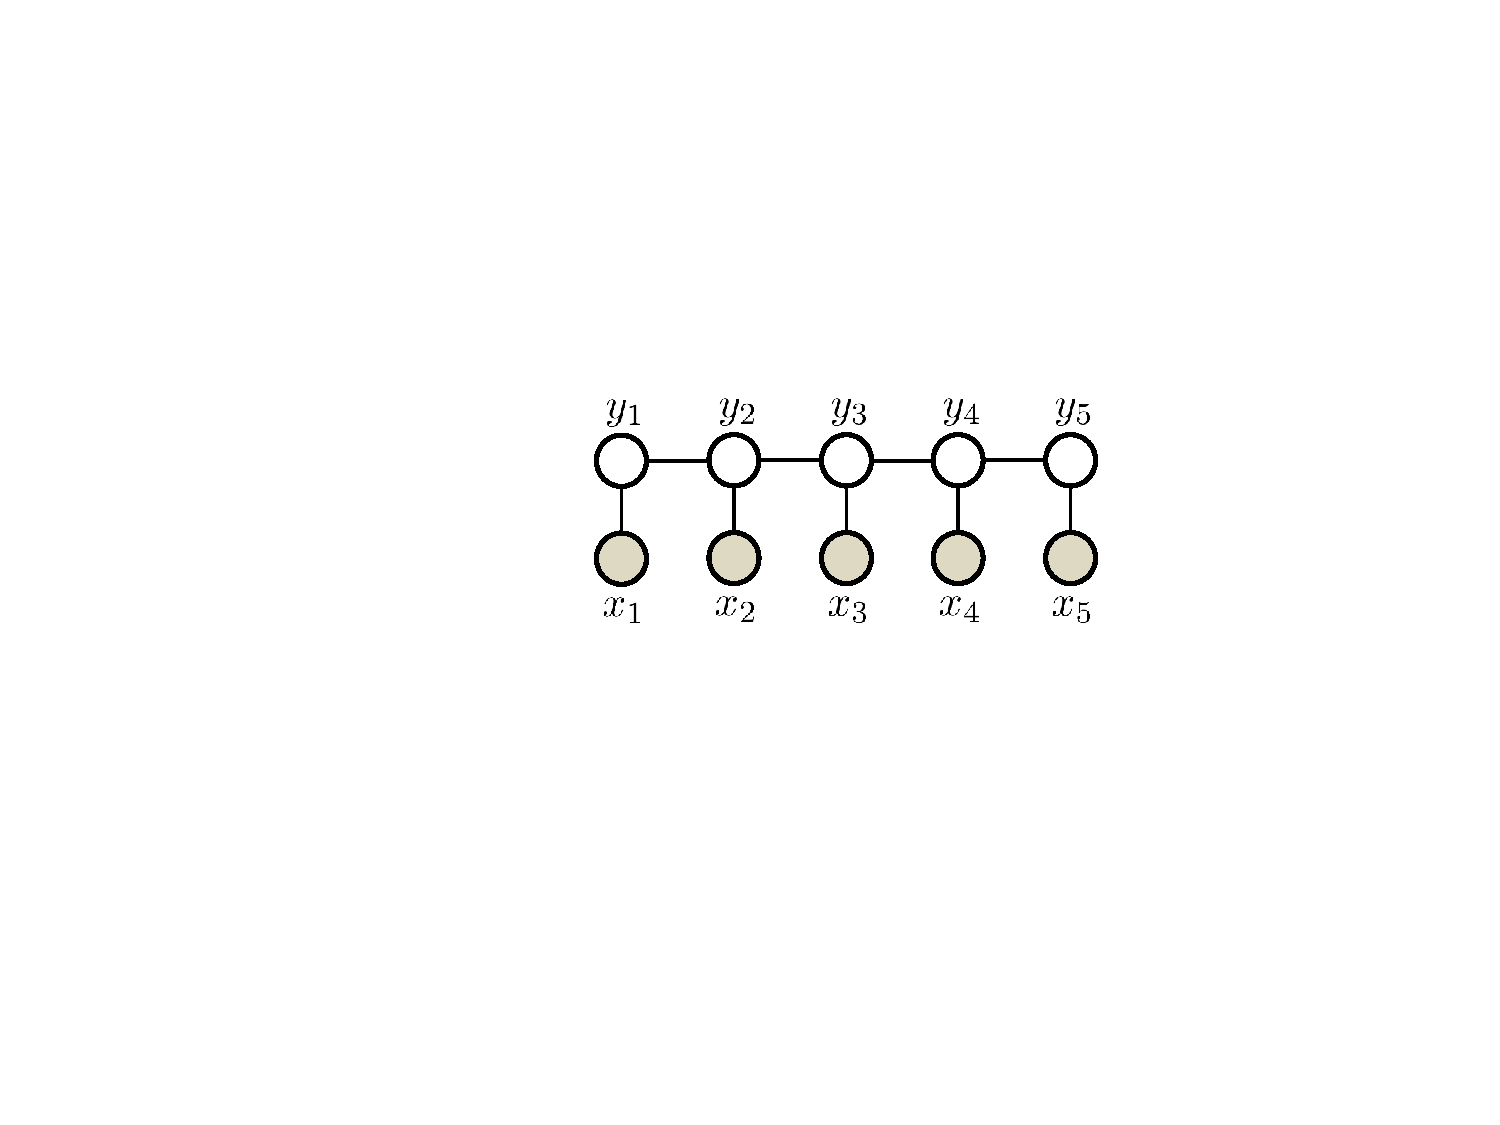
\includegraphics[width=5cm]{crf}
  \caption{CRF for word-letter}\label{fig:CRF_model}
\end{minipage}
\end{figure}








\paragraph{Dataset}
The original dataset is downloaded from \href{http://www.seas.upenn.edu/~taskar/ocr/}{http://www.seas.upenn.edu/$\sim$taskar/ocr}.
It contains the image and label of 6,877 words collected from 150 human subjects,
with 52,152 letters in total.
To simplify feature engineering, each letter image is encoded by a 128 (=16*8) dimensional vector,
whose entries are either 0 (black) or 1 (white).

\begin{center}
	\fbox{\begin{minipage}{38em}
			The PETSc code that loads the data always appends a constant 1 to the feature vectors,
			leading to \underline{129} features in total.
			Make sure your own SGD implementation also includes this additional feature.
			This is different from Project 1.
	\end{minipage}}
\end{center}

The 6,877 words are divided evenly into training and test sets,
and the package provides two versions of data files under the folder \verb#data/#:
\begin{itemize}
	\item For PETSc experiments, the files are \verb#train_petsc.txt#, \verb#test_petsc.txt#, and a file that describes the fields: \verb#fields_petsc.txt#.
	\item For SGD and ADAM experiments, the files are \verb#train_sgd.txt#, \verb#test_sgd.txt#, and a file that describes the fields:  \verb#fields_sgd.txt#.
	Note they are the same as \verb#train.txt#, \verb#test.txt#, and \verb#fields_crf.txt# used in Project 1, and they are just renamed to avoid confusion.
\end{itemize}


Note in this dataset, only lowercase letters are involved, \ie\ 26 possible labels.
Since the first letter of each word was capitalized and the rest were in lowercase,
the dataset has removed all first letters.


\paragraph{Performance measures}
%
We will compute two error rates: \emph{letter-wise} and \emph{word-wise}.
Prediction/labeling is made on at letter level,
and the percentage of incorrectly labeled letters is called letter-wise error.
A word is correctly labeled if and only if \emph{all} letters in it are correctly labeled,
and the word-wise error is the percentage of words in which at least one letter is mislabeled.


\section{Conditional Random Fields}

Suppose the training set consists of $n$ words.
The image of the $t$-th word can be represented as
$X^t = (\xvec^t_1, \ldots, \xvec^t_m)^\top$,
where $t$ is a superscript (not exponent) and each \emph{row} of $X^t$ is a letter.
Here $m$ is the number of letters in the word,
and $\xvec^t_j$ is a 129 dimensional vector that represents its $j$-th letter image.
To ease notation, we simply assume all words have $m$ letters,
and the model extends naturally to the general case where the length of word varies.
The sequence label of a word is encoded as
$\yvec^t = (y^t_1, \ldots, y^t_m)$,
where $y^t_k \in \Ycal := \{1, 2, \ldots, 26\}$ represents the label of the $k$-th letter.
So in Figure \ref{fig:brace}, $y^t_1 = 2$, $y^t_2 = 18$, \ldots, $y^t_5 = 5$.

Using this notation, the Conditional Random Field (CRF) model for this task is a sequence shown in Figure \ref{fig:CRF_model},
and the probabilistic model for a word/label pair $(X, \yvec)$ can be written as
\begin{align}
\label{eq:crf}
  p(\yvec | X ) &= \frac{1}{Z_X} \exp \rbr{\sum_{s=1}^m \inner{\wvec_{y_s}}{\xvec_s} + \sum_{s=1}^{m-1} T_{y_s, y_{s+1}}} \\
  \where Z_X &= \sum_{\hat{\yvec} \in \Ycal^m} \exp \rbr{\sum_{s=1}^m \inner{\wvec_{\yhat_s}}{\xvec_s} + \sum_{s=1}^{m-1} T_{\yhat_s, \yhat_{s+1}}}.
\end{align}
%
%$Z(X)$ is a normalization constant depending on $X$.
$\inner{\cdot}{\cdot}$ denotes inner product between vectors.
Two groups of parameters are used here:

\begin{itemize}
\item {\bf Node weight:} Letter-wise discriminant weight vector $\wvec_k \in \RR^{128}$ for each possible letter label $k \in \Ycal$;
\item {\bf Edge weight:} Transition weight matrix $T$ which is sized $26$-by-$26$.
$T_{ij}$ is the weight associated with the letter pair of the $i$-th and $j$-th letter in the alphabet.  For example $T_{1,9}$ is the weight for pair (`a', `i'), and $T_{24,2}$ is for the pair (`x', `b'). In general $T$ is not symmetric, \ie\ $T_{ij} \neq T_{ji}$, or written as $T' \neq T$ where $T'$ is the transpose of $T$.
\end{itemize}
Given these parameters (\eg\ by learning from data), the model \eqref{eq:crf} can be used to predict the sequence label (\ie\ word) for a new word image $X^* := (\xvec^*_1, \ldots, \xvec^*_m)^\top$ via the so-called maximum a-posteriori (MAP) inference:
\begin{align}
  \label{eq:crf_decode}
  \yvec^* = \argmax_{\yvec \in \Ycal^m} p(\yvec | X^*)
  = \argmax_{\yvec \in \Ycal^m} \cbr{ \sum_{j=1}^m \inner{\wvec_{y_j}}{\xvec^*_j} + \sum_{j=1}^{m-1} T_{y_j, y_{j+1}}}.
\end{align}

Finally, given a training set $\{X^t, \yvec^t\}_{t=1}^n$ ($n$ words),
we can estimate the parameters $\{\wvec_k : k \in \Ycal\}$ and $T$ by maximum a posteriori over the conditional distribution in \eqref{eq:crf}, or equivalently
\begin{align}
\label{eq:obj_MLE}
  \min_{\{\wvec_k\}, T} \ -\frac{1}{n}\sum_{t=1}^n \log p(\yvec^t | X^t) + \frac{\lambda}{2} \rbr{\sum_{k \in \Ycal} \nbr{\wvec_k}^2 + \sum_{ij} T^2_{ij}}.
\end{align}
Here $\lambda > 0$ is a trade-off weight that balances log-likelihood and regularization.
\begin{center}
	\fbox{\begin{minipage}{38em}
			Here we place the adjustable weight $\lambda$ on the regularizer,
			while in Project 1 we put the adjustable weight $C$ on the negative log-likelihood.			
	\end{minipage}}
\end{center}

\subsection{Gradient formula}

For a single word-label pair $(X^t, \yvec^t)$,
it is not hard to derive the formulae of $\grad_{\wvec_k} \log p(\yvec^t|X^t)$ and $\grad_{T_{ij}} \log p(\yvec^t|X^t)$, \ie\ the gradient of $\log p(\yvec^t|X^t)$ with respect to $\wvec_k$ and $T_{ij}$.
Here $i$, $j$, $k$ all range in $\Ycal$, indexing the classes (possible label of letters).
By \eqref{eq:crf},
%
\begin{align}
\label{eq:log_prob}
  \log p(\yvec^t | X^t) = -\log Z_{X^t} + \sum_{s=1}^m \inner{\wvec_{y_s^t}}{\xvec^t_s} + \sum_{s=1}^{m-1} T_{y_s^t, y_{s+1}^t}.
\end{align}
%
{\bf Step 1.} Let us first compute $\grad_{\wvec_k} \log p(\yvec^t|X^t)$,
and to this end we start with the gradient of the first term $\log Z_{X^t}$.
Denote $\sembrack{x} = 1$ if $x$ is true, and 0 otherwise.
Then
%
\begin{align}
  \grad_{\wvec_k} \log Z_{X^t}
    &= \frac{1}{Z_{X^t}} \grad_{\wvec_k} Z_{X^t} \\
    &= \frac{1}{Z_{X^t}} \sum_{\yvec \in \Ycal^m} \grad_{\wvec_k} \exp \rbr{\sum_{s=1}^m \inner{\wvec_{y_s}}{\xvec^t_s} + \sum_{s=1}^{m-1} T_{y_s, y_{s+1}}} \\
    &=\frac{1}{Z_{X^t}} \sum_{\yvec \in \Ycal^m} \exp \rbr{\sum_{s=1}^m \inner{\wvec_{y_s}}{\xvec^t_s} + \sum_{s=1}^{m-1} T_{y_s, y_{s+1}}}
    \rbr{\sum_{s=1}^m \inner{\grad_{\wvec_k} \wvec_{y_s}}{\xvec^t_s} + \grad_{\wvec_k} \sum_{s=1}^{m-1} T_{y_s, y_{s+1}}} \\
    &= \sum_{\yvec \in \Ycal^m} p(\yvec | X^t) \sum_{s=1}^m \sembrack{y_s = k} \xvec^t_s \\
\label{eq:grad_marginal}
    &= \sum_{s=1}^m p(y_s = k | X^t) \xvec^t_s.
\end{align}

So it requires the marginal distribution of each node $y_s$ given $X^t$.
Note in \eqref{eq:grad_marginal}, $p(y_s = k | X^t)$ means $y_s$ is a random variable.
We do not write $p(y_s^t = k | X^t)$ since $y_s^t$ is the given label.
Of course it \emph{is} valid to write $p(y_s = y^t_s | X^t)$.
The derivative of the second term in \eqref{eq:log_prob} with respect to $\wvec_k$ is simply
%
\begin{align}
  \grad_{\wvec_k} \sum_{s=1}^m \inner{\wvec_{y^t_s}}{\xvec^t_s} = \sum_{s=1}^m \sembrack{y^t_s = k} \xvec^t_s.
\end{align}

So in total, for a single sequence/word $X^t=(\xvec^t_1, \ldots, \xvec^t_m)^\top$ with label $\yvec^t \in \Ycal^m$,
we have
\begin{align}
  \grad_{\wvec_k} -\log p(\yvec^t|X^t) &= \sum_{s=1}^m ( p(y_s = k | X^t) - \sembrack{y^t_s = k}) \xvec^t_s,
\end{align}
which can be compactly written in a matrix form as
\begin{align}
\label{eq:def_Gt}
  G^t &:= -(\grad_{\wvec_1} \log p(\yvec^t|X^t), \ldots, \grad_{\wvec_{26}} \log p(\yvec^t|X^t))
  = (X^t)^\top C^t \in \RR^{129 \times 26}, \\
\label{eq:def_Ct}
  \where C^t &\in \RR^{m \times 26} \quad \text{and} \quad C_{sk} =  p(y_s = k | X^t) - \sembrack{y^t_s = k}.
\end{align}
%
We will call $C^t$ the {\underline c}oefficient matrix.
If we further stack all training \emph{words} into
\begin{align}
\label{eq:train_collect}
  \yvectr := \begin{pmatrix} \yvec^1 \\ \vdots \\ \yvec^n \end{pmatrix} \in \RR^{mn},
  \qquad
  \Xtr := \begin{pmatrix} X^1 \\ \vdots \\ X^n \end{pmatrix} \in \RR^{mn \times 129},
  \qquad
  \Ctr := \frac{1}{n} \begin{pmatrix} C^1 \\ \vdots \\ C^n \end{pmatrix} \in \RR^{mn \times 26},
\end{align}
then the aggregated average gradient can be written as
\begin{align}
\label{eq:def_gradient}
  G_{\text{train}} := \frac{1}{n} \sum_{t=1}^n G^t &= -\frac{1}{n} \rbr{\grad_{\wvec_1} \sum_{t=1}^n \log p(\yvec^t|X^t), \ldots, \grad_{\wvec_{26}} \sum_{t=1}^n \log p(\yvec^t|X^t)}
  = \Xtr^\top \Ctr.
\end{align}
%
This will be exactly the formula used in our PETSc implementation,
modulo some matrix replication trick that will be detailed in Section \ref{sec:data_loading}.
All we need to do is to compute the $\Ctr$ matrix,
where the key quantity is the marginal distributions $p(y_s = k | X^t)$.
That requires dynamic programming and the cost $O(m \abr{\Ycal}^2)$ for each word.

{\bf Step 2.} We next compute $\grad_{T_{ij}} \log p(\yvec^t|X^t)$.
Running the above derivation analogously, we derive
\begin{align}
\label{eq:grad_edge_weight}
  \grad_{T_{ij}} -\frac{1}{n} \sum_{t=1}^n \log p(\yvec^t | X^t) = \frac{1}{n} \sum_{t=1}^n \sum_{s=1}^{m-1} \cbr{p(y_s=i, y_{s+1} = j | X^t) - \sembrack{y^t_s = i \text{ and } y^t_{s+1} = j} }.
\end{align}
%
Our code will compute these quantities explicitly, and the key challenge here is to compute the edge marginals $p(y_s=i, y_{s+1} = j | X^t)$.
They can be computed together with the node marginals in Step 1,
with the overall computational cost being $O(m \abr{\Ycal}^2)$ for each word.

\subsection{IID model}

If we treat all letter images as IID (independent and identically distributed) samples,
then the model \eqref{eq:crf} can be simplified by fixing $T_{ij}$ to 0.
As a result, the node marginals can be trivially computed by
\begin{align}
  p(y_s = k | X^t) = \exp(\inner{\wvec_k}{\xvec^t_s}) \bigg/ \sum_{k' = 1}^{26} \exp(\inner{\wvec_{k'}}{\xvec^t_s}).
\end{align}
%
The gradient formulae (for $\wvec_k$) in (\ref{eq:def_Gt}, \ref{eq:def_gradient}) remain unchanged.
Of course, we do not need the gradient in $T_{ij}$ any more.


\section{Parallel Optimization: Implementation Details and Facilities Provided}
\label{sec:parallel_detail}

You do not have to work from scratch.
The following routines have been provided in the folder \verb!code_PETSc!,
allowing you to focus on optimization.
In my own implementation, only {\bf 100 lines} of new code were needed to complete the implementation of CRF!
And it's C++ code, not Matlab!
Of course, you will need to read and digest a lot of code before being able to fill in the blanks.
To help you get familiar with the PETSc functions that are important for this project,
a demo program \verb!demo_PETSc.cpp! is provided, and we will refer to its functions later.
To run the demo with two cores, just type

\verb!make demo!

\vspace{-0.5em}
\verb!mpirun -n 2 ./demo_PETSc!

Currently, the code can run IID training which
treats each letter image as an independent training example and learns a 26-class classifier.
To run the IID training with 2 cores, copy \verb!train.txt! and \verb!test.txt! to the current directory,
and then type

\verb!make!

\vspace{-0.5em}
{\small
\verb!mpirun -n 2 ./seq_train -data ./train.txt -tdata ./test.txt -lambda 1e-3 -loss IID -tol 1e-3!
}
\vspace{-1em}

The meaning of the command line arguments are:

\vspace{-1em}
\begin{itemize}[itemsep=0mm]
  \item \verb!./train.txt!: the training data filename,
  \item \verb!./test.txt!: the test data filename,
  \item \verb!-lambda!: the value of the $\lambda$ in \eqref{eq:obj_MLE},
  \item \verb!-tol!: the tolerance for optimization termination,
  \item \verb!-loss!: must be \verb!IID! or \verb!CRF!.
\end{itemize}
\vspace{-1em}

A sample_dataset console printout is given in \verb!sample_out_IID.txt!.
To switch to CRF training AFTER completing your implementation,
just change the last \verb!IID! into \verb!CRF!.
The code currently dumps the following performance metrics to STDOUT at each iteration:

{\small
\verb!iter fn.val gap time feval.num  train_lett_err  train_word_err  test_lett_err  test_word_err!
}

\vspace{-1em}
They stand for:
\vspace{-1em}
\begin{enumerate}[itemsep=0mm]
  \item the current iteration number,
  \item the objective value of the current solution,
  \item some measure indicating the distance from optimality, \eg\ square of the gradient norm, duality gap, etc,
  \item the number of times that the callback function (of objective and gradient) has been called,
  \item letter-wise error rate on the training data (out of 100),
  \item word-wise error on the training data,
  \item letter-wise error on the test data,
  \item word-wise error on the test data.
\end{enumerate}




\subsection{Data loading}
\label{sec:data_loading}

The data is loaded into the application context structure ``\verb!AppCtx user!" in the \verb!main! function (line 39 of \verb!seq_train.cpp!).
Go to \verb!appctx.hpp! to peruse the fields and detailed comments on the \verb!SeqCtx! and \verb!AppCtx! structures.
The vector \verb!labels! records $\yvectr$ (the labels of the letters in the training data),
and the matrix \verb!data! \emph{corresponds to} the training data matrix $\Xtr$
(but not exactly; see the matrix replication below).
Their definitions follow \eqref{eq:train_collect} exactly.
Note in C++, array indices start from 0.
So the labels (the values in the \verb!labels! vector) are encoded from 0 to 25.
We also added a constant 1 to each image feature vector,
and therefore each $\xvec^t_s \in \RR^{129}$ ($\Xtr$ has 129 columns).

In parallel computing, it is important to specify the range of rows and columns that belong to each process.
We allow PETSc to apply its own heuristics to partition the columns.
However we must take control over the row boundaries (letters),
because we do not want any word to be split into multiple processes.
So we first evenly divided the 6,877 \emph{words} throughout the processes,
and then all letters of each word must go to the same process.
As a result, when computing the node and edge marginal distributions,
each process can process its own set of local words independently.

To record the range of words stored in my process, as well as the number of letters in each word,
a structure \verb!SeqCtx! is introduced in \verb!appctx.hpp!.
It records word related information, \eg\ what is the (global) index of the first and last word/letter stored in this process, what is the length of each word (\#letters).
Detailed comments have been attached to this structure in \verb!appctx.hpp!.
Make sure you understand it.


The job of loading the data into the \verb!AppCtx! structure is implemented in
\verb!loaddata_libsvm.cpp/hpp!.
But {\bf you do NOT need to read any line in it}.
Just focus on the code of optimization by directly using the resulting label vector,
data matrix, and sequence contexts.

The last important technique we exploited is the \emph{virtual} replication of the data matrix $\Xtr$,
using the PETSc function MatCreateMAIJ.
This is highly effective and cool.
Recall to compute the model output for $\xvec^t_s$, we need to compute $\inner{\xvec^t_s}{\wvec_k}$.
PETSc allows us to compute all these numbers (all $t, s, k$) by a \emph{single} matrix-vector multiplication
(equivalent to the matrix-matrix multiplication in \eqref{eq:def_gradient}, but differ in implementation).
To avoid writing a for-loop with 26 iteration,
PETSc allows us creates a new matrix that replicates $\Xtr$ for 26 times:

\verb!MatCreateMAIJ!($\Xtr$, 26, $\Xnew$)

Of course $\Xnew$ does NOT physically replicate $\Xtr$;
it just takes a note in its data structure, and the repetition is only logical.
If we query its size by MatGetSize, it is 26 times of that of $\Xtr$ in both rows and columns.
In \verb!loaddata_libsvm.cpp!, we did first create $\Xtr$, and then call \verb!MatCreateMAIJ!.
The local \#row and \#column of $\Xnew$ is also 26 times of those of $\Xtr$.
However, $\Xnew$ is NOT really equal to replicating $\Xtr$ 26 times in both row and column directions
(making a $26$-by-$26$ block matrix).
The only property we need to understand about $\Xnew$ is the result when it is multiplied with a vector.
Here is the detailed explanation.

In TAO (indeed most existing solvers), the optimization variable must be a vector (not a matrix).
So our solution is to collect all weight entries into a long vector ($26 \cdot 129$ dimensional).
For some reason that will become clear later, we do NOT just concatenate $\{\wvec_k\}$ into
$(\wvec_1^\top, \ldots, \wvec_{26}^\top)^\top$.
Instead it uses the \emph{row-major} representation of the matrix $(\wvec_1, \wvec_2, \ldots, \wvec_{26})$:
%
\begin{align}
\label{eq:vec_w}
  \wvec := \begin{pmatrix}
    w_{1,1} \\ w_{2,1} \\ \vdots \\ w_{26, 1} \\
    w_{1,2} \\ w_{2,2} \\ \vdots \\ w_{26, 2} \\
    \vdots \\
    w_{1,129} \\ w_{2,129} \\ \vdots \\ w_{26, 129}
  \end{pmatrix}
  \qquad
  \where w_{k,d} \text{ is the } d\text{-th entry of } \wvec_k.
\end{align}
%
Since C++ uses row-major and PETSc is based on C++,
this choice is not surprising.
Here it can be seen that the index of class (1 to 26) runs first,
followed by the index of features (1 to 129).
If you really wonder why such an order is adopted, here is a sketch reason.
The layout of $\wvec$ in \eqref{eq:vec_w} allows the local range of columns of $\Xtr$ to be directly mapped to the local range of elements in $\wvec$.
Suppose the first 11 columns of $\Xtr$ belong to process 0, and the next 12 columns belong to process 1.
Then we can naturally determine the layout of the entries in $\wvec$ by
assigning the first $11 \cdot 26$ entries to process 0,
and the next $12 \cdot 26$ entries to process 1.
Recall that the vector entries belonging to a process must be {\bf contiguous (cannot jump)}.
If we assemble $\{\wvec_k\}$ into $(\wvec_1^\top, \ldots, \wvec_{26}^\top)^\top$,
then this natural correspondence of local range will no longer be available.

The most appealing consequence of this design is that the product of $\Xnew$ and $\wvec$ is very nice:
\begin{align}
\label{eq:mat_vec_result}
  \Xnew \cdot \wvec \qquad \text{ produces } \qquad
  \begin{pmatrix}
    \inner{\xvec^1_1}{\wvec_1} \\
    \inner{\xvec^1_1}{\wvec_2} \\
    \vdots \\
    \inner{\xvec^1_1}{\wvec_{26}} \\
    \inner{\xvec^1_2}{\wvec_1} \\
    \vdots \\
    \inner{\xvec^1_2}{\wvec_{26}} \\
    \vdots \\
    \inner{\xvec^1_m}{\wvec_{26}} \\
    \vdots \\
    \inner{\xvec^n_m}{\wvec_{26}}
  \end{pmatrix},
\end{align}
%
which is exactly the row-major representation of the matrix
$\Xtr \cdot (\wvec_1, \wvec_2, \ldots, \wvec_{26})$.

{\bf Take this as a DEFINITION} resulting from the logical replication of $\Xnew$,
and do NOT try to find a matrix representation of $\Xnew$ that yields this result.
If you really wonder why it is defined in such a way, consider once again the local storage/partitioning.
In \eqref{eq:mat_vec_result}, the index of class (1 to 26) again runs first,
then the letter index within a word (subscript of $\xvec$),
and finally the word index (superscript of $\xvec$).
This is extremely useful,
because the result is automatically consistent with our design principle that
the local partitioning is based on dividing the \emph{word set} evenly.
So if we put the first 15 words on process 0 (\ie\ $15m$ rows of $\Xtr$),
then here the first $15 \cdot m \cdot  26$ entries of the resulting product in \eqref{eq:mat_vec_result} will reside on process 0.
In consequence, when a process accesses its local chunk of the vector via \verb!VecGetArray!,
it will directly obtain the $\inner{\xvec^t_s}{\wvec_k}$ for all the words $t$ belonging to itself.
This is the key benefit of using \verb!MatCreateMAIJ!,
and it saves considerable inter-process communication
(imagine otherwise we will have to send the elements in the product to their rightful process).
This multiplication is performed in line 73 of \verb!iid_loss.cpp!.

\cprotect\fbox{
  \begin{minipage}{16cm}
In \verb!appctx.hpp!, the matrix variable \verb!data! in the \verb!AppCtx! structure
is already $\Xnew$,
\ie\ already replicated logically for 26 times.
So is the test data matrix \verb!tdata!.
  \end{minipage}
}

To see how many words/letter are allocated to my process, check the following line in \verb!iid_loss.cpp!:

\vspace{-0.5em}
\verb!ierr = MatGetLocalSize(user->data, &m_local, &dim_local);!
\vspace{-0.5em}

The value of \verb!m_local! is 26 times the number of local letters.
The (global) indices of the first and last local words are \verb!user->seq.wBegin! and \verb!user->seq.wEnd!, respectively.
These indices start from 0, and \verb!user->seq.wEnd! is indeed one plus the last index,
so that the number of local words is \verb!user->seq.wEnd - user->seq.wBegin!,
and a for loop can be written as

\vspace{-0.25em}
\verb!for (i = user->seq.wBegin; i < user->seq.wEnd; i++)!
\vspace{-0.25em}

The number of letters in each word can be found in \verb!user->seq.wLen[]!,
using the \emph{global} index.
See more details in \verb!appctx.hpp!.


\subsection{Implementation of IID modeling}

The implementation of IID modeling has been provided to illustrate the relevant usage of TAO and PETSc.
It is recommended to peruse \verb!iid_loss.cpp!.


The multiplication of data matrix with model vector in \eqref{eq:mat_vec_result} is done in the following line of \verb!iid_loss.cpp!:

\vspace{-0.25em}
\verb!ierr = MatMult(user->data, w, user->fx);!
\vspace{-0.25em}

The resulting vector is stored in the \verb!user->fx! variable.
Then it calls the function \verb!loss_coef! to compute $p(y_s = k | X^t)$.
As explained above, the local entries of \verb!user->fx! will automatically encompass all the values $\inner{\xvec^t_s}{\wvec_k}$ over $k \in \Ycal$, $s \in \{1,\ldots,m\}$, and $t$ (word index) over the local words.
These are sufficient for the local process to compute the node probabilities $p(y^t_s = k)$.
It is furthermore sufficient for CRF to compute the node and edge probabilities,
because for each word these quantities can be computed without accessing other words.

The function \verb!loss_coef! computes $p(y_s = k | X^t)$,
storing the results in the vector \verb!user->c_node!:

\vspace{-0.4em}
\verb!ierr = loss_coef(user->fx, user->labels, user->c_node, f, user, &user->seq);!
\vspace{-0.4em}

More accurately, it only computes $p(y_s = k | X^t)$ for the local letters,
and stores the results in the \emph{local memory} of the vector \verb!user->cnode!.
Here the $t$ index only covers the local words.
Since it is doing IID modeling,
one can simply enumerate over all local letters, ignoring their membership in words.
Hence in line 33 of \verb!iid_loss.cpp!, it directly loops over the letter,
rather than using a two-level loop (first over the words and then over the letters in each word).
For each letter, it grabs $26$ entries from \verb!user->fx!
(or called \verb!fx_array! inside the \verb!loss_coef! function),
computes the probabilities,
and then appends the results to \verb!cnode_array!.
Suppose the local range of words is from $t_1$ to $t_2$.
Then upon completion, \verb!cnode_array! contains entries
\begin{align}
\label{eq:def_c_local}
  \cvec_{\text{local}} :=
    \frac{1}{n}
    \begin{pmatrix}
    p(y_1 = 1 | X^{t_1}) \\
    \vdots \\
    p(y_1 = 26 | X^{t_1})  \\
    p(y_2 = 1| X^{t_1})  \\
    \vdots \\
    p(y_2 = 26 | X^{t_1})   \\
    \vdots \\
    p(y_m = 26 | X^{t_1})   \\
    \vdots \\
    p(y_m = 26 | X^{t_2})
  \end{pmatrix}
  -
  \frac{1}{n}
  \begin{pmatrix}
    \sembrack{y^{t_1}_1 = 1} \\
    \vdots \\
    \sembrack{y^{t_1}_1 = 26} \\
    \sembrack{y^{t_1}_2 = 1} \\
    \vdots \\
    \sembrack{y^{t_1}_2 = 26} \\
    \vdots \\
    \sembrack{y^{t_1}_m = 26} \\
    \vdots \\
    \sembrack{y^{t_2}_m = 26}
  \end{pmatrix}
\end{align}

This is again nice because the entries are naturally arranged in the order.
Finally to compute the gradient according to (\ref{eq:def_Gt}, \ref{eq:def_gradient}),
we only need to compute $\Xnew^\top * \cvec$ (line 88 of \verb!iid_loss.cpp!).
This is really neat, and the reasoning is left as an exercise
(just re-apply the definition in \eqref{eq:mat_vec_result}).

For numerical robustness, the following trick is widely used when computing $\log \sum_i \exp(x_i)$ for a given array of real numbers $\{x_i\}$.  If we naively compute and store $\exp(x_i)$ as intermediate results, underflow and overflow could often occur.  So we resort to computing an equivalent form $M + \log \sum_i \exp(x_i - M)$, where $M := \max_i x_i$.  This way, the numbers to be exponentiated are always non-positive (eliminating overflow), and one of them is 0 (hence underflow is not an issue).  Similar tricks can be used for computing $\exp(x_1) / \sum_i \exp(x_i)$.


\subsection{Suggestions on CRF implementation}

Compared with the IID model,
the CRF introduces the edge weights $T_{ij}$.
Since we still need to represent the optimization variable as a vector, we have to concatenate the node weights and edge weights.
So the new optimization variable is
\begin{align}
\label{eq:wedges}
  \wcrf :=
  \begin{pmatrix}
    \wnode\\
    \wedges
  \end{pmatrix}
  \where
  \wnode \text{ is as in \eqref{eq:vec_w}},
  \quad \text{and} \quad
  \wedges =
   \begin{pmatrix}
    T_{1,1} \\
    \vdots \\
    T_{1, 26} \\
    T_{2, 1} \\
    \vdots \\
    T_{2, 26} \\
    \vdots \\
    T_{26, 26}
  \end{pmatrix}.
\end{align}

Then at each iteration we will first need to extract the $\wvec$ part for nodes, and then the $T$ part.
PETSc does provide tools to extract sub-vectors,
but let us do it with a simple hack.
Obviously,
\begin{align}
  \wnode \quad := \quad \underbrace{ \begin{pmatrix}
    1 &   &   &   & \ldots & \ldots \\
     & 1 &   &   & \ldots & \ldots \\
     & & \ddots &  & \ldots & \ldots \\
     &  &  & 1 & \ldots & \ldots
  \end{pmatrix}}_{:= M_1} \wcrf
\end{align}
where in $M_1$ all elements \emph{not} set to 1 take the value 0.
The size of $M_1$ can be easily inferred from the length of $\wcrf$ and the $\wvec$ in \eqref{eq:vec_w}.
Similarly, we have
\begin{align}
  \wedges
  \quad = \quad \underbrace{ \begin{pmatrix}
    \ldots & \ldots & 1 &   &   &    \\
     \ldots & \ldots & & 1 &   &   & \\
     \ldots & \ldots & & & \ddots &  & \\
    \ldots & \ldots & &  &  & 1 &
  \end{pmatrix}}_{:= M_2} \wcrf
\end{align}
Trivially, we can recover $\wcrf$ from $\wnode$ and $\wedges$ by using the transpose of $M_1$ and $M_2$:
\begin{align}
\label{eq:combine_transpose}
  \wcrf = M_1^\top \wnode + M_2^\top \wedges.
\end{align}
In fact, you may use \eqref{eq:combine_transpose} to compute the \emph{gradient} of $\wcrf$ by first computing the gradients in $\wnode$ and $\wedges$ (called \verb!g_node! and \verb!g_edge! in the \verb!AppCtx! structure respectively), and then concatenate them by multiplying with $M_1^\top$ and $M_2^\top$ as in \eqref{eq:combine_transpose}.
The PETSc function MatMultTranspose can be useful here.
In \verb!crf_loss.cpp!, the line

\verb!ierr = make_sparse_matrix(&user->M1, *w, user->w_node, 0);!

has allocated the $M_1$ matrices with the proper size (similarly for $M_2$),
and you can directly use them.
Since these are extremely sparse matrices, the multiplications above are indeed very efficient.

Since $\wedges$ is needed for all processes to compute the node and edge marginal distributions,
it needs to be broadcast to all processes.
Since $\wedges$ is a distributed vector,
one needs to use the scatter utility in PETSc,
so that all elements residing on other processes will be copied to my process,
and vice versa.
This is readily facilitated by the \verb!VecScatterCreateToAll! function,
and the demo code \verb!demo_PETSc.cpp! shows how to use it.
The \verb!w_edgeloc! variable in \verb!AppCtx! is a local vector (called sequential by PETSc),
storing the \emph{entire} $\wedges$ locally.

Given $\Xnew * \wnode$ (as in IID) and $\wedges$,
we need to compute the node and edge marginal distributions,
so that they can be further used to compute he gradients in $\wnode$ and $\wedges$ by
(\ref{eq:def_Gt}, \ref{eq:def_gradient}) and \eqref{eq:grad_edge_weight} respectively.
The efficient computation here requires dynamic programming,
and the code has been provided.  See Section \ref{sec:inference}.

Finally, after all processes complete computing the gradients on the edge weights,
they need to be summed up as in \eqref{eq:grad_edge_weight}.
This can again be done by the scatter, but using the \verb!ADD_VALUES! argument.
See again \verb!demo_PETSc.cpp!.



\subsection{Inference}
\label{sec:inference}

The following inference routines have been provided with the package.

{\bf 1. The MAP inference} in \eqref{eq:crf_decode} has been implemented in the \verb!get_errors! function in \verb!crf_loss.cpp!.
In fact, this function does more;
it returns (by setting via call-by-reference) the letter-wise and word-wise errors
(\verb!lError! and \verb!wError!).
It takes three vectors/arrays as input:

\vspace{-1em}
\begin{itemize}
  \item \verb!fx!: the $\Xnew * \wvec$ in \eqref{eq:mat_vec_result},
and the caller (function \verb!Evaluate!) needs to invoke the multiplication.  \verb!get_errors! needs to be called twice, once for the training data, and once for the test data (change $\Xnew$ to \verb!user->tdata!).
  %
  \item \verb!labels!: simply \verb!user->labels!.
  %
  \item \verb!w_edgeloc!: a vector that encodes the entire $\wedges$.  It should be a sequential vector, not distributed.  It collects \emph{all} the elements of $\wedges$, and stores them in a vector in my process.
      See how it is created in \verb!AllocateWorkSpace! via \verb!VecScatterCreateToAll! (\verb!crf_loss.cpp!).
\end{itemize}
\vspace{-1em}

Both \verb!fx! and \verb!labels! are distributed vectors,
and the function \verb!get_errors! extracts their \emph{local} elements by \verb!VecGetArray!.


{\bf 2. The marginal inference} for $p(y_s = k | X^t)$ and $p(y_s = i, y_{s+1}=j | X^t)$ is performed by \verb!loss_coef! in \verb!crf_loss.cpp!.
It takes three inputs and produces two outputs.
The inputs are \verb!fx!, \verb!labels!, and \verb!w_edgeloc!,
which are all identical to those in the above \verb!get_errors! function.

Outputs (set via call-by-reference):

\vspace{-1em}
\begin{itemize}
  \item \verb!c_node!: the $\cvec_{\text{local}}$ vector in \eqref{eq:def_c_local}, and it has already done the division by $n$.  It is a distributed vector, and \verb!loss_coef! only sets its local elements.
  %
  \item \verb!g_edgeloc!: a $26^2$ dimensional vector that encodes this process' contribution to the gradient of $\wedges$ (cf. \eqref{eq:grad_edge_weight} and \eqref{eq:wedges}).
      Concretely, if the process hosts words from $t_1$ to $t_2$, then it gives
      \begin{align}
        \frac{1}{n} \sum_{t=t_1}^{t_2} \sum_{s=1}^{m-1} \cbr{p(y_s=i, y_{s+1} = j | X^t) - \sembrack{y^t_s = i \text{ and } y^t_{s+1} = j} }.
      \end{align}
      Note \verb!g_edgeloc! has already done the division by $n$.
      It is a sequential vector (not distributed), and all processes have its own copy.
      The caller \verb!LossGrad! needs to sum them up to form the true gradient stored in a distributed fashion.  This can be done by scatter as explained above.
\end{itemize}
\vspace{-1em}

\subsection{Other miscellaneous}

A timer class is included to facilitate the measurement of computational cost.
The implementation is in \verb!timer.cpp! and \verb!timer.hpp!.
You definitely do NOT need to read these two files.
Just check how the three timers are used in \verb!seq_train.cpp!
(the \verb!wallclock_total! field) and \verb!iid_loss.cpp! (start and stop).

TAO can be terminated in many different ways, and users can set it easily.
For example, reaching the maximum number of iterations or function evaluation,
falling below some threshold of gradient norm or step size.
See \verb!seq_train.cpp! for some sample_dataset usage.

In very rare cases, the program crashes with strange runtime errors (e.g. returning \verb!nan!).
Then try a clean re-compiling by ``\verb!make clean!" followed by ``\verb!make!".

\section{Parallel Optimization: Tasks for Experiment}

First complete the implementation of CRF based on the given framework.
{\bf The implementation should be filled into \verb!crf_loss.cpp! and \verb!crf_loss.hpp!},
especially the two functions \verb!LossGrad! and \verb!Evaluate!.
New functions and variables can be added there.
If you create new files, then the \verb!makefile! will need to be updated.

Then answer the following questions in your report.
We will use P1, P2, etc to label the questions for the parallel optimization experiment.
S1, S2, etc will be used for the stochastic optimization experiment.

{\bf Question P1.}
Run your CRF implementation using the following command

{\small
\verb!mpirun -n 3 ./seq_train -data ./train.txt -tdata ./test.txt -lambda 1e-3 -loss CRF -tol 1e-3!
}
\vspace{-1em}

Copy and paste to your report
i) the first 11 lines (\ie\ 10 iterations) of the output,
and
ii) the last line when it converges.
%
For example (extracted from \verb!sample_out_IID.txt!)

\vspace{-1em}
\begin{verbatim}
iter fn.val gap time feval.num train_lett_err train_word_err test_lett_err test_word_err
0 24.5949 4.51757 0.259464 1 92.309174 100.000000 92.220780 100.000000
1 20.3838 4.97532 0.687281 3 71.683428 100.000000 71.745935 100.000000
2 17.6704 3.53674 0.793315 4 67.556737 99.883653 67.318116 99.941844
3 15.7212 2.60525 0.897278 5 55.165106 98.283886 55.141614 98.255307
4 13.858 2.06517 1.1684 6 48.117751 97.207679 48.244141 96.888630
5 11.8215 2.43501 1.40405 7 43.459330 94.560791 43.999542 94.765920
6 10.527 1.11771 1.51042 8 37.968636 91.128563 38.556378 91.596394
7 10.0913 0.820058 1.6166 9 36.219320 89.470622 36.911215 90.375109
8 9.44112 0.820068 1.71968 10 33.210034 86.823735 34.380487 88.107008
9 9.10282 1.64436 1.82459 11 33.129118 86.474695 34.059852 86.827566
10 8.69891 0.656452 1.92768 12 30.763303 83.449680 31.758149 84.210526
:
:
107 6.24397 0.00412999 15.8922 112 20.221169 68.499127 22.944500 73.480663
Optimization converged with status CONVERGED_GTTOL.
\end{verbatim}

Note the command line controls termination by \verb!-tol 1e-3!.
See line 75 of \verb!seq_train.cpp! for its meaning.
In my implementation, the program terminated after 95 iterations,
with a word-wise test error of 49.52 and objective value 3.3395.
If you would like to further confirm the correctness,
run your code from Project 1 on this dataset and compare the optimal objective value.
Recall that we now use 129 features, so we can't directly copy the result from Project 1.
Also note that the LBFGS solver implemented in PETSc/Matlab/Python can be different,
so they can be different in many aspects although the optimal objective value should be close.

\rule{\paperwidth}{0.6pt}
{\bf Answer P1.}
The first eleven lines (10 iterations) of the output as well as the last line when it converges:
\begin{verbatim}
iter fn.val gap time feval.num train_lett_err train_word_err test_lett_err test_word_err
0 24.5949 4.55704 0.480855 1 92.309174 100.000000 92.220780 100.000000
1 20.2619 5.09505 1.91933 3 71.379031 100.000000 71.421483 100.000000
2 17.428 3.65693 2.64741 4 66.666667 99.825480 66.382930 99.883687
3 15.3061 2.66886 3.37782 5 53.446615 97.643979 53.500267 97.702821
4 13.2133 2.13058 4.0924 6 45.382037 96.160558 45.644706 95.347485
5 10.8931 2.51846 4.8255 7 39.671714 91.826643 40.426750 92.294272
6 9.33426 1.1719 5.5542 8 33.803414 87.085515 34.647683 87.699913
7 8.75664 0.875296 6.28745 9 31.553192 84.293194 32.326895 85.199186
8 7.89758 0.851361 7.01093 10 28.551613 80.337405 29.361020 81.913347
9 7.2986 1.54779 7.7407 11 27.129812 77.370564 28.128101 78.045944
10 6.79134 0.731165 8.45953 12 24.552075 72.949389 25.608825 74.469322
:
:
114 3.07372 0.00436801 87.6235 120 10.545987 39.383362 14.268265 48.706019
Optimization converged with status CONVERGED_GTTOL.
\end{verbatim}

{\bf Question P2.}
The test error obviously depends on the regularization parameter $\lambda$. For each $\lambda$ value in \verb!{1e-2, 1e-4, 1e-6}!, plot a figure with a single curve where the x-axis is the CPU time elapsed (in seconds), and the y-axis is the objective value of the current solution.
One dot for each iteration's output.
Again use three cores, and CRF loss.
If it takes too long to converge,
you may relax the tolerance to \eg\ \verb!-tol 1e-2!,
or set the max number of iteration or function evaluation to some smaller value
(line 77 and 79 of \verb!seq_train.cpp!),
provided that the trend has leveled off.

Does a larger value of $\lambda$ allow the optimization to converge faster in CPU time,
or a smaller value of $\lambda$?  Why?
Hint: the solver is quasi-Newton (like LBFGS).

\rule{\paperwidth}{0.6pt}
{\bf Answer P2.} A larger value of $\lambda$ constrains the objective function due to its behavior as a regularizer, therefore, as $\lambda$ increases, the constraints on the possible solutions increases. Due to the use of line search in LBFGS, a more constrained problem requires a fewer number of function evaluations. Therefore, the optimizer converges on the solution faster.

\begin{figure}[t]
\centering
\subfigure[$\lambda =$ {\sf 1e-2}]{
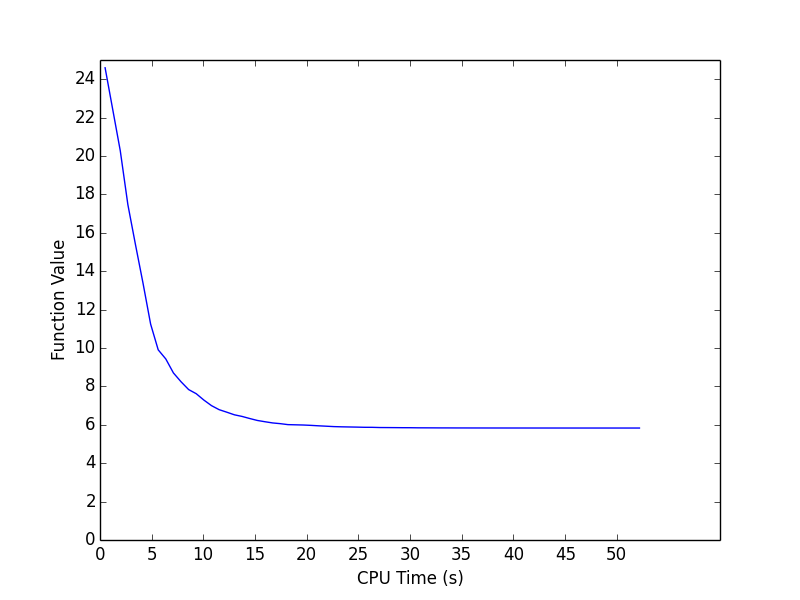
\includegraphics[width=5.8cm]{q2-a}}
~~
\subfigure[$\lambda =$ {\sf 1e-4}]{
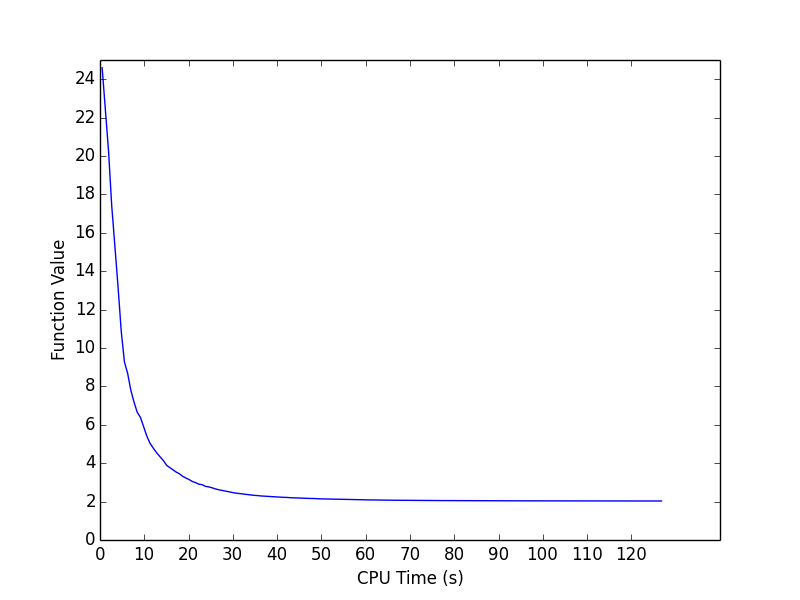
\includegraphics[width=5.8cm]{q2-b}}
~~
\subfigure[$\lambda =$ {\sf 1e-6}]{
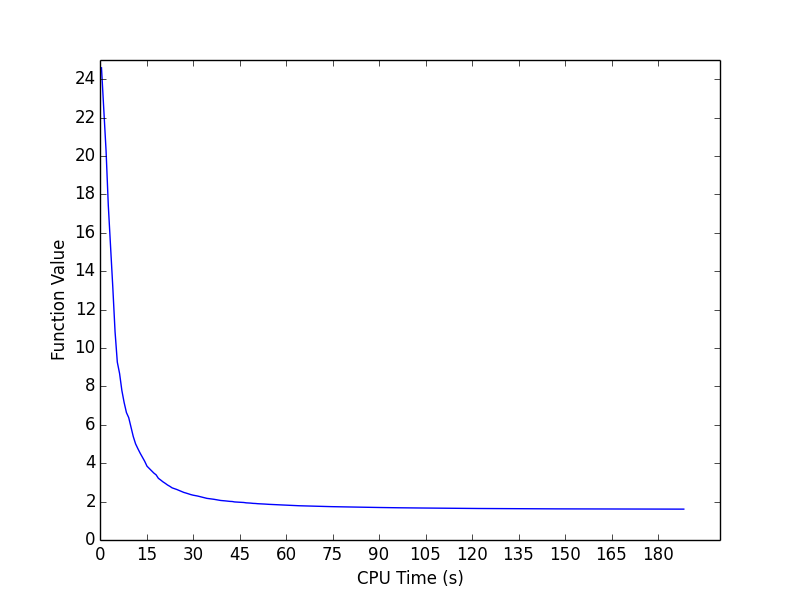
\includegraphics[width=5.8cm]{q2-c}}
\caption{Comparison between $\lambda \in \{${\sf 1e-2, 1e-4, 1e-6}\}.}
\label{fig:compare_sgd}
\end{figure}

{\bf Question P3.}
Pick the $\lambda$ from the last question that gives the lowest test word-wise error.
Plot a figure with two curves:
one for the test letter-wise error as time goes by (x-axis is CPU time in seconds),
and one for the training letter-wise error.
Then plot another figure for word-wise error.
Made-up plots are shown in Figure \ref{fig:letter_err} and \ref{fig:word_err}.

What can be observed from these plots?
In addition, compare these plots with those in Question P2.
Does training/test error keep decreasing as the objective function is being reduced?

\rule{\paperwidth}{0.6pt}
{\bf Answer P3.} One main observation is that the margin between the training/test Word-wise error is much larger than the margin between the training/test Letter-wise error. When compared to the plots in P2, we can see that as the objective function value decreases, the training/test error keeps decreasing till an extent. The errors do not decrease after a certain point and just hover around a value. The decrease in training/test error and function value is quite correlated to an extent.

\begin{figure}[t]
	\centering
	\begin{minipage}[t]{0.49\textwidth}
		\centering
		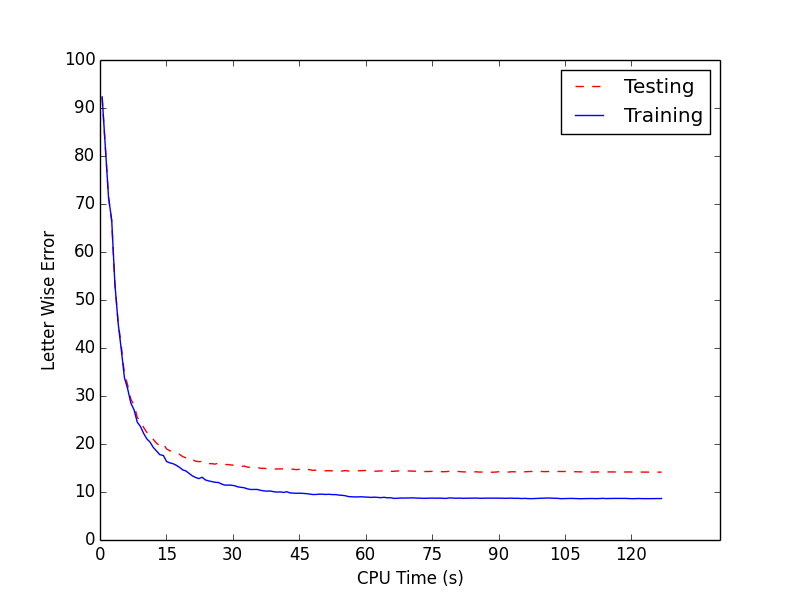
\includegraphics[width=5.8cm]{q3-a}
		\caption{Letter-wise error v.s. CPU time ($\lambda$=1e-4)}
		\label{fig:letter_err}
	\end{minipage}
	%
	\begin{minipage}[t]{0.49\textwidth}
		\centering
		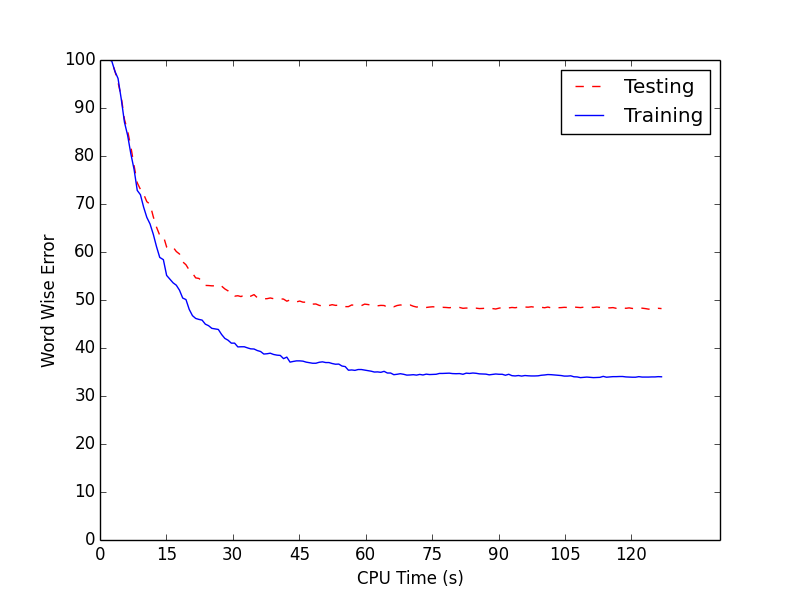
\includegraphics[width=5.8cm]{q3-b}
		\caption{Word-wise error v.s. CPU time ($\lambda$=1e-4)}
		\label{fig:word_err}
	\end{minipage}
\end{figure}

{\bf Question P4.}
Scalability test.
In parallel computing, it is standard to study how the speedup depends on the number of cores.
Suppose some job costs $T_r$ time if run on $r$ cores.
Then the speedup of $r$ cores is defined as $T_1 / T_r$.
To rigorously define the ``time to converge",
one approach is to first set the tolerance to very tight (\eg\ \verb! -tol 1e-5!)
and get a highly accurate estimate of the true minimum objective value.
Denote it as $f^* \ge 0$.
Then for any given new parameter setting of the solver (the optimization problem itself is kept intact), define the ``time to converge" as the time required to find an solution whose objective value falls below $1.01 \cdot f^*$ (or  $1.001 \cdot f^*$, etc).

%\begin{figure}[t]
%	\centering
%	\begin{minipage}[t]{0.49\textwidth}
%		\centering
%		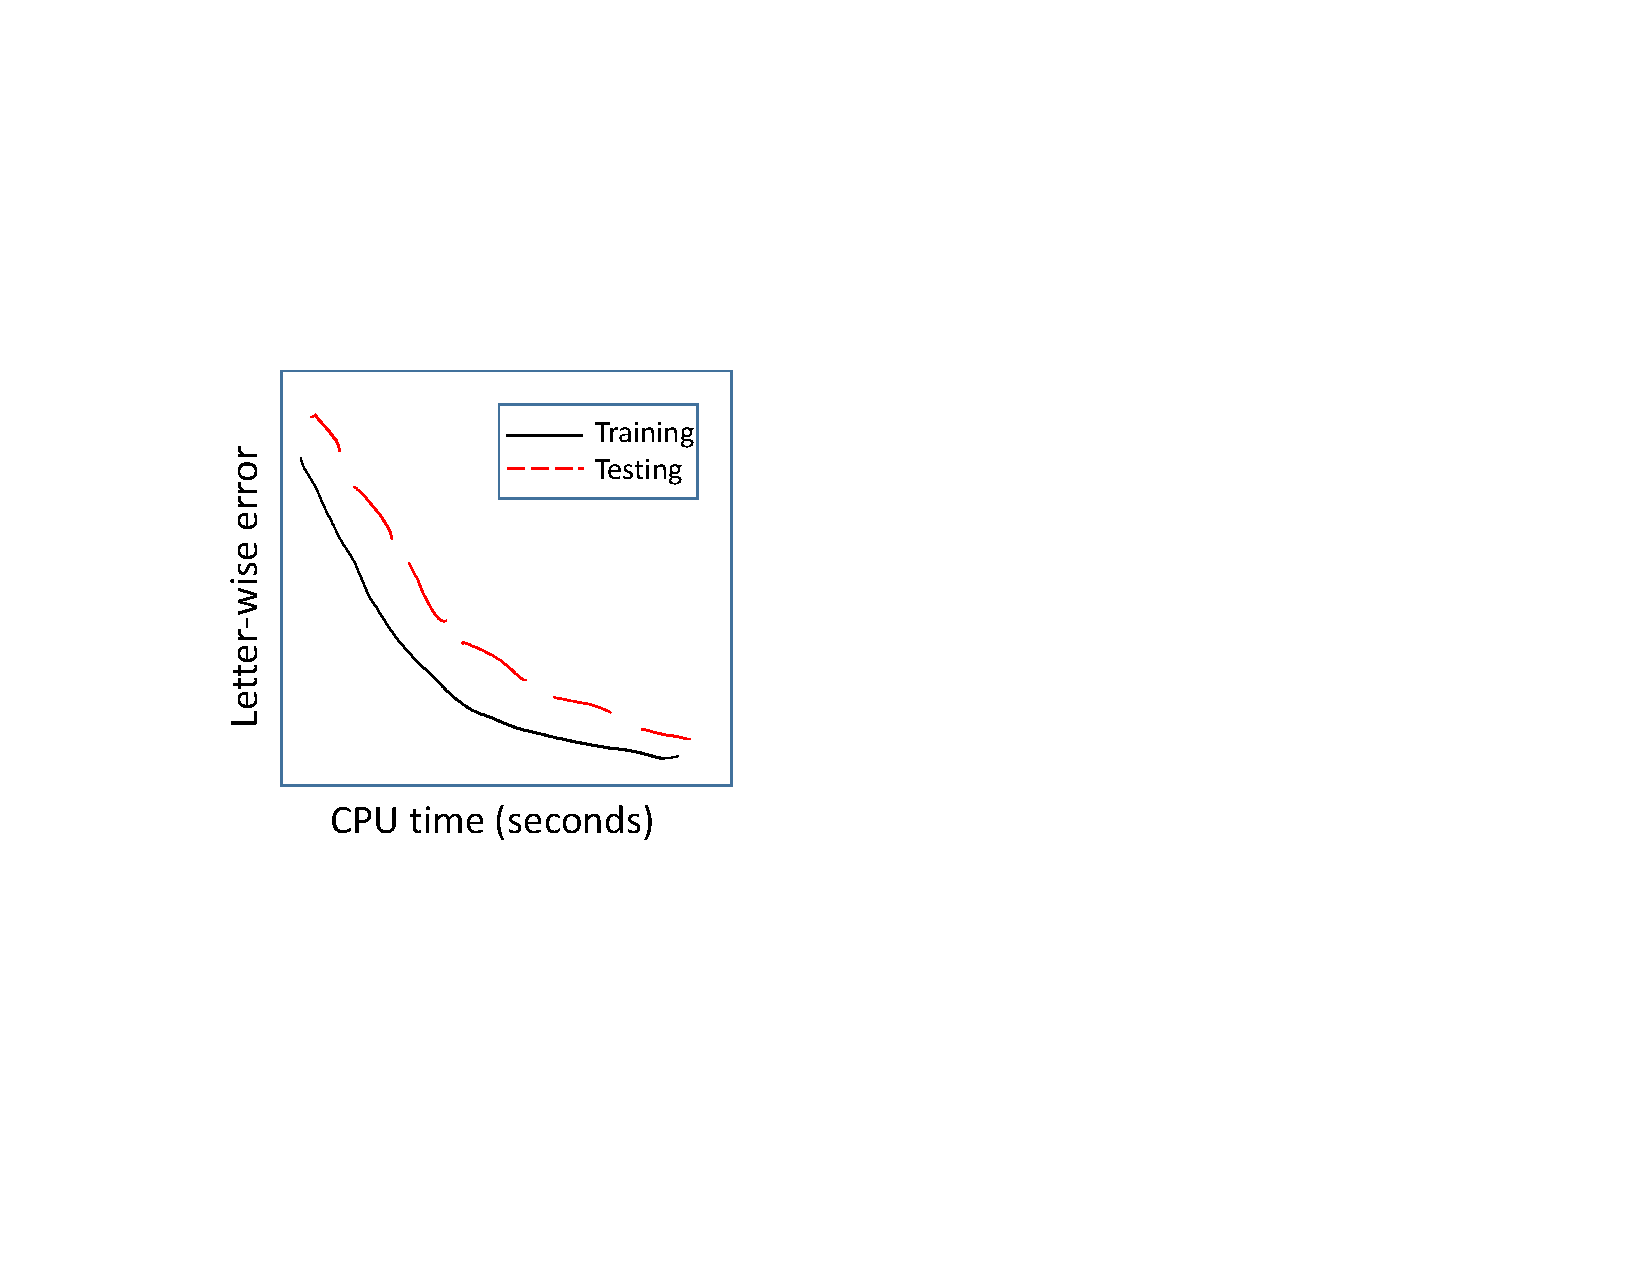
\includegraphics[width=5cm]{curve_letter}
%		\caption{Letter-wise error v.s. CPU time ($\lambda$=???)}
%		\label{fig:letter_err}
%	\end{minipage}
%	%
%	\begin{minipage}[t]{0.49\textwidth}
%		\centering
%		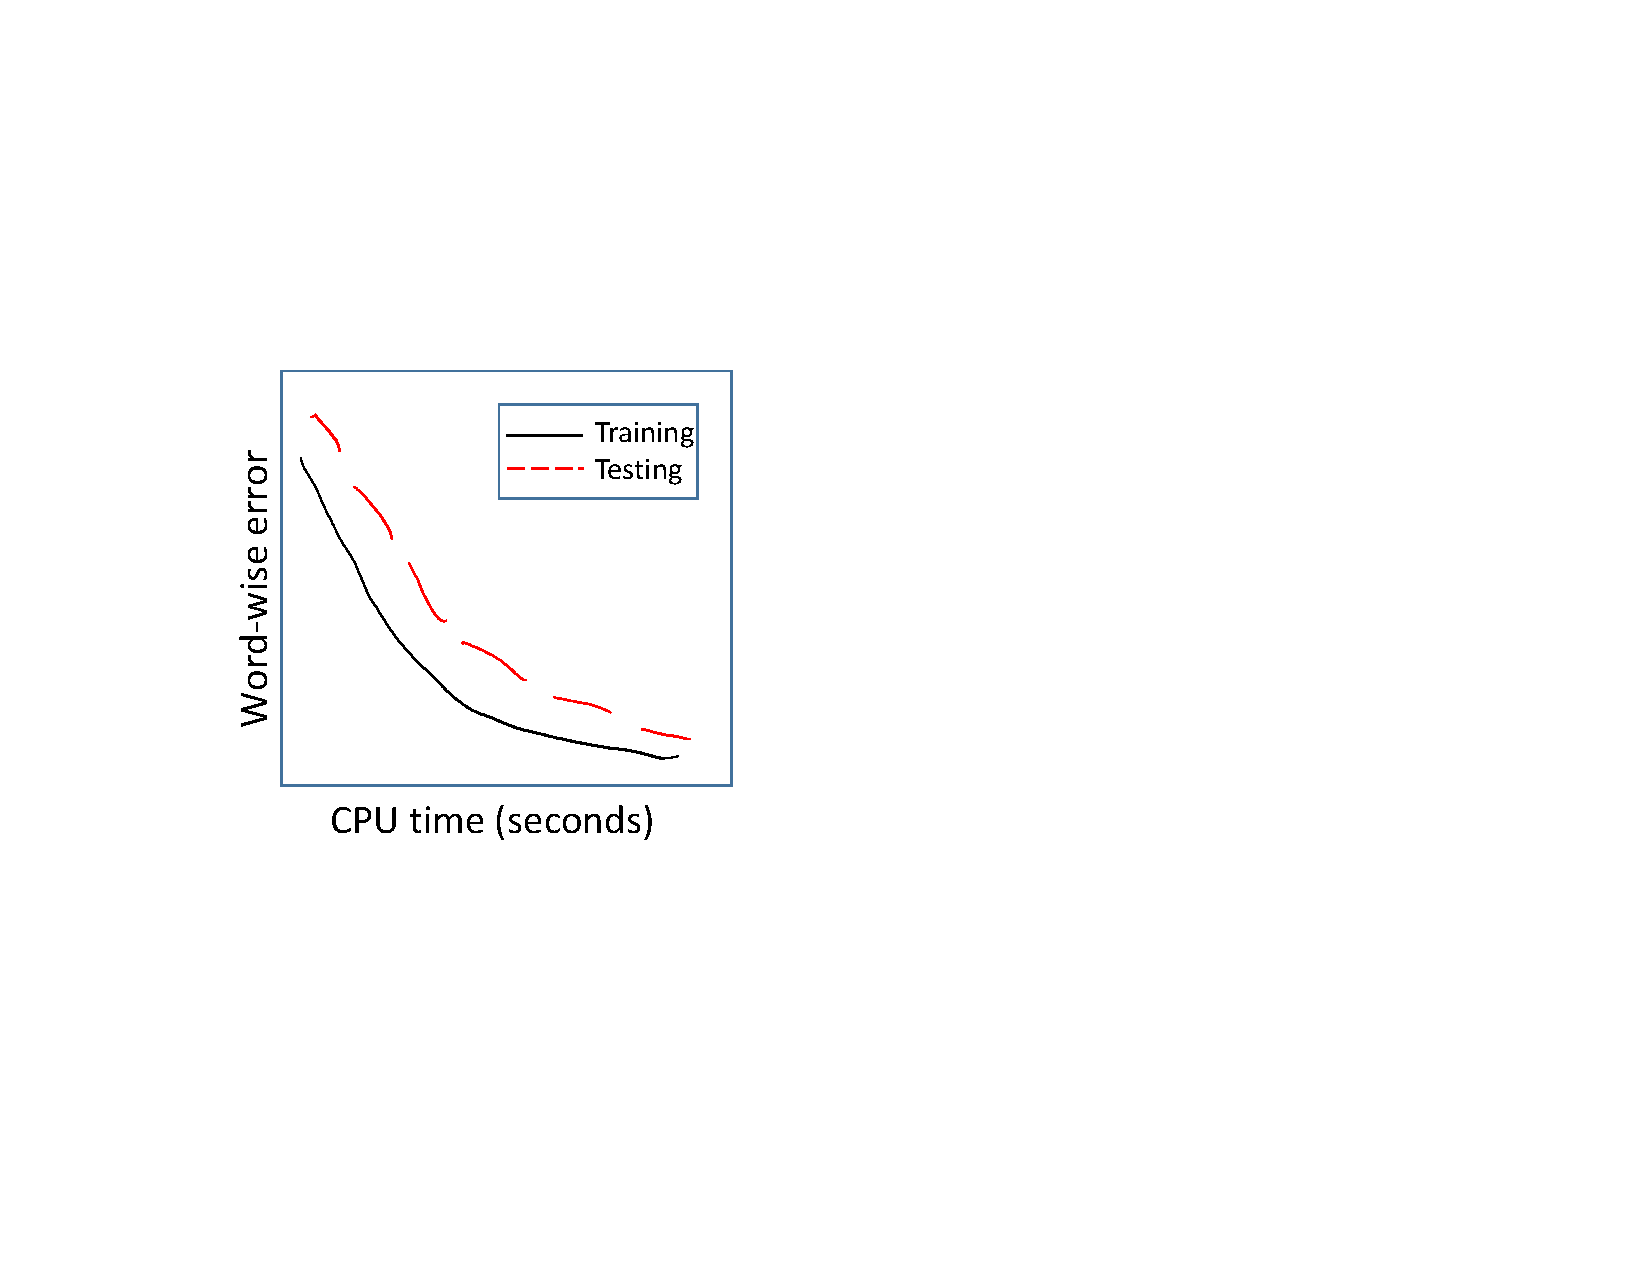
\includegraphics[width=5cm]{curve_word}
%		\caption{Word-wise error v.s. CPU time ($\lambda$=???)}
%		\label{fig:word_err}
%	\end{minipage}

%\end{figure}
%
%\begin{figure}[htbp!]
%\vspace{2em}
%\centering
%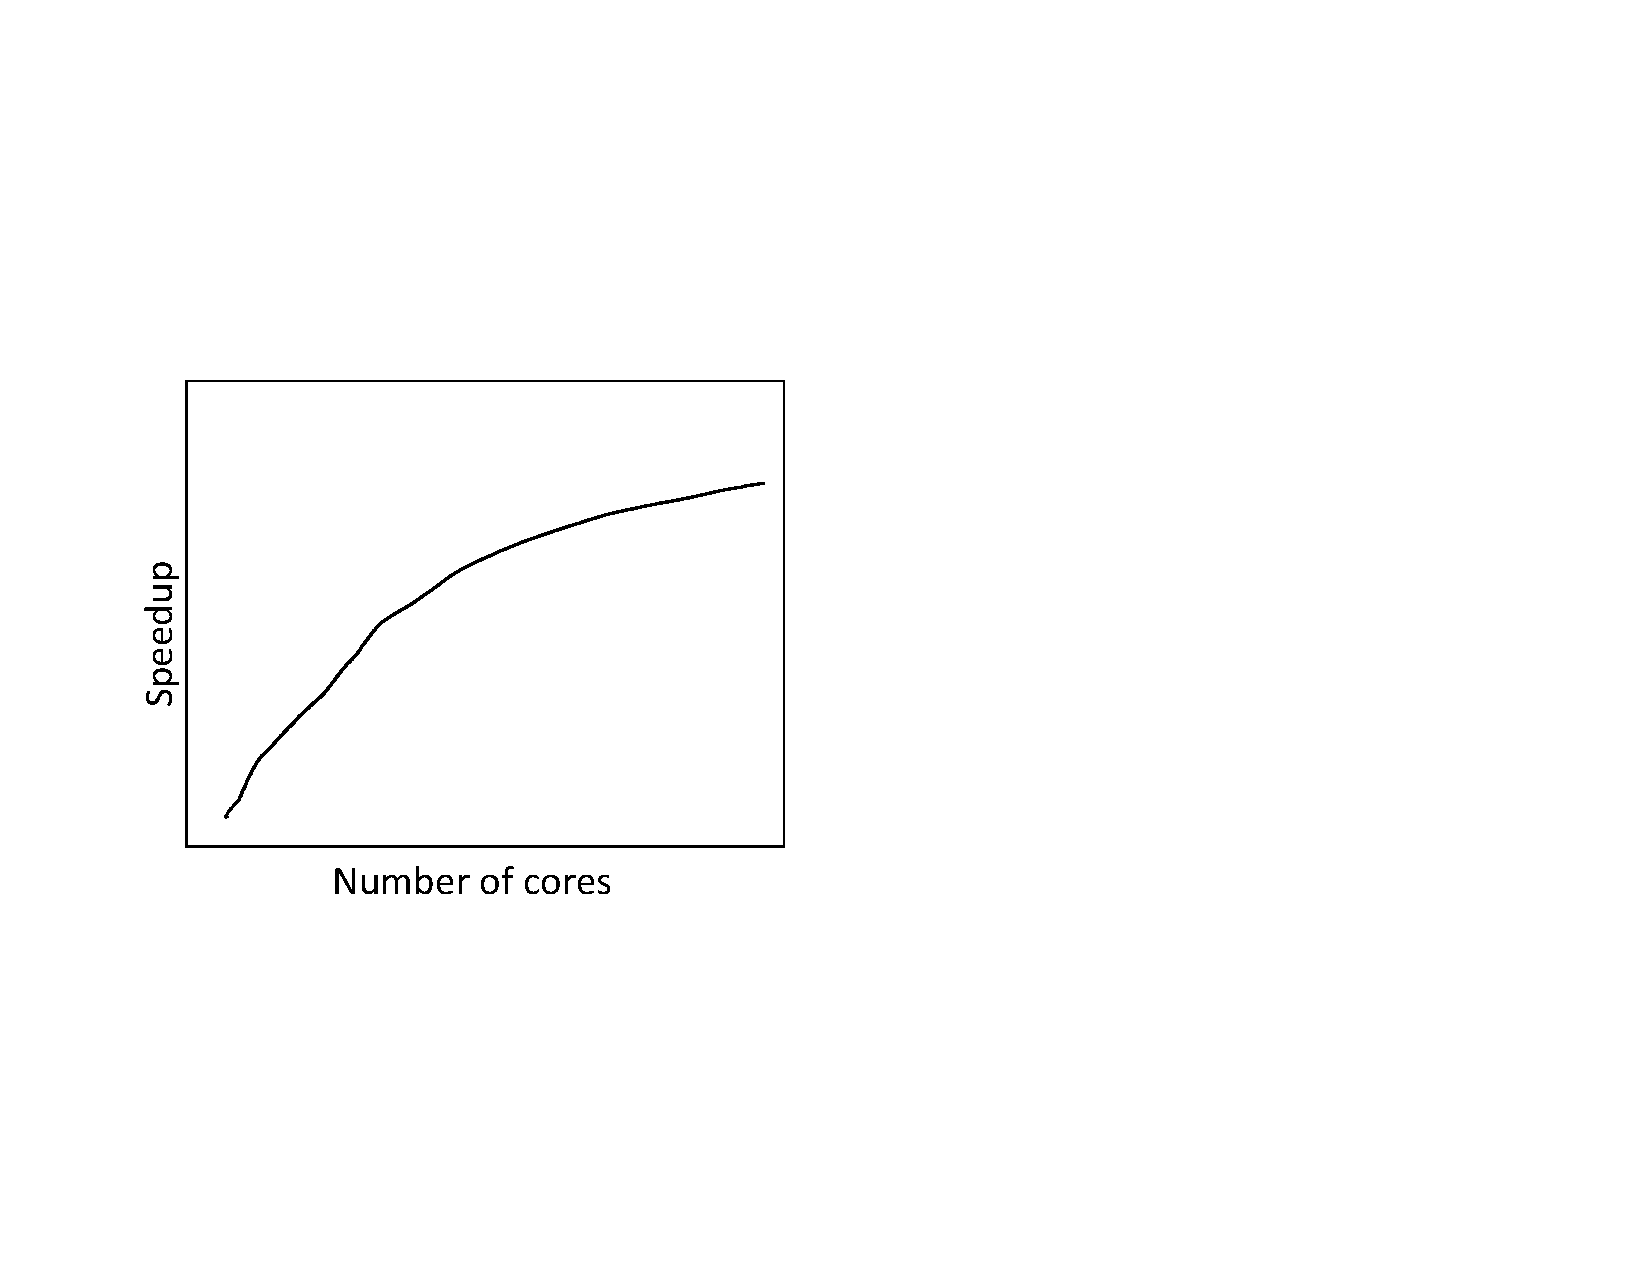
\includegraphics[width=5.8cm]{scalability}
%\caption{Speedup as a function of \#core}
%\label{fig:scalability}
% \end{figure}

Fix \verb!-lambda 1e-4 -loss CRF!.
Vary the number of core $r \in \{1, 2, 4, 6, 8\}$ and plot a curve of $T_1 / T_r$ as a function of $r$.
A made up figure is given in Figure \ref{fig:scalability}.
You may use 8 cores to first get a highly accurate estimate $f^*$ with \verb!-tol 1e-5!.
When $r$ is small, it will take longer, and you may relax the tolerance to ``\verb!-tol 1e-3!" provided that the solver does not terminate before finding a solution whose objective value is less than $1.01 \cdot f^*$ (or $1.001 \cdot f^*$ if you feel proper).

Based on the plot, what conclusion can be drawn?
If the curve is not linear, explain why.

\rule{\paperwidth}{0.6pt}
{\bf Answer P4.} Based on the plot, one can deduce the curve is not linear. This indicates that the speedup with respect to the \textit{\# of cores} and \textit{speedup factor} is \textbf{sublinear speedup}. This observation is common and expected. The speedup is NOT linear because of factors such as \textit{overhead} and \textit{contention for resources}. If there were none, we could expect a \textbf{linear speedup}. If we have the case:

$$S(p) = \frac{T_{s}}{T_{par}(p)}$$

where:

$T_{s} = $ time to converge with 1 core and $T_{par}(p) = $ time to converge with p cores. If \textit{S(p) = p}, then we have linear speedup. Also, the speedup has to obey Amdahl's Law. Thus, this observation is consistent with said theory.

\begin{figure}
\centering
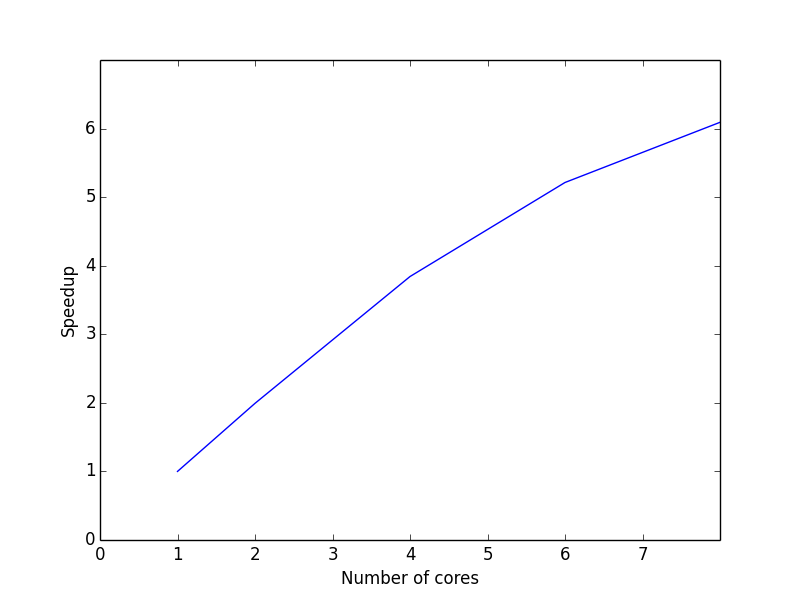
\includegraphics[width=8cm]{q4}
\caption{Speedup as a function of \#core}
\label{fig:scalability}
\end{figure}

{\bf Question P5.}
Do we really need to store the whole $\Ctr$ matrix in memory (cf. \eqref{eq:train_collect}) via storing $\cvec_{\text{local}}$ over all processes (cf. \eqref{eq:def_c_local})?
If yes, explain why.
If no, explain how this can be saved and how the computational performance will be impacted.

\rule{\paperwidth}{0.6pt}
{\bf Answer P5.} The answer is \textbf{yes}, we need to store the whole $\Ctr$ matrix in memory (cf. \eqref{eq:train_collect}) via storing $\cvec_{\text{local}}$ over all processes (cf. \eqref{eq:def_c_local}). This restriction is placed because when calculating $\cvec_{\text{local}}$, we cannot scatter the values over all workers as we need to sequentially perform the gradient calculation depending on the value from the previous word.

\section{Comparison with Stochastic Optimization}

We next compare LBFGS (as we used in PETSc) with two stochastic optimization algorithms: SGD and ADAM.
You need to implement SGD and ADAM in your favorite languages (probably the one you used in Project 1).
{\bf Remember that our input $\xvec_i$ for each letter is now augmented with a constant 1, hence having 129 features.}
Since you have already implemented the gradient computation in Project 1, 
you can directly use it,
with the obvious adaption that SGD/ADAM only needs the gradient on a single word rather than over the entire training set.
Don't forget to test the routine again by using \verb#gradest# or equivalent.


The result of LBFGS can be just copied from the PETSc results.
However, its timing was based on running on the cluster with multiple cores,
and is therefore not comparable with that of SGD/ADAM which use a single core.
So instead of comparing in terms of CPU time, 
we resort to the \emph{effective number of passes}, 
i.e., how many passes the solvers have swept over the entire training set.
For LBFGS, it is the 5-th number (integer) in the printout shown in {\bf Question P1}.
For SGD/ADAM, it is the number of words sampled so far divided by 3438
(\#words in the training set).

For the two stochastic methods, each update (based on a randomly sampled word) is cheap, 
much cheaper than measuring the performance,
e.g., the training objective of CRF in \eqref{eq:obj_MLE}, or the two types of error on the test set.
So you can choose to compute these measures every 1000 update, 
or pick a frequency that you feel reasonable.



Answer the following questions in your report.

{\bf Question S1.}
%
Now for each $\lambda \in$ \verb!{1e-2, 1e-4, 1e-6}!,
plot a figure that compares the three methods (LBFGS, SGD, ADAM) over the training objective value.
See Figure \ref{fig:compare_sgd} for made-up plots,
where the x-axis uses the effective number of passes.
{\bf You may tune the parameters of SGD/ADAM} (but not LBFGS/PETSc),
such as step size, exponential decay rate, etc.
Use whatever parameter that you feel is good for the solver on this problem,
and mention them in the report.
What conclusion can be drawn from these figures?



\begin{figure}[t]
\centering
\subfigure[$\lambda =$ {\sf 1e-2}]{
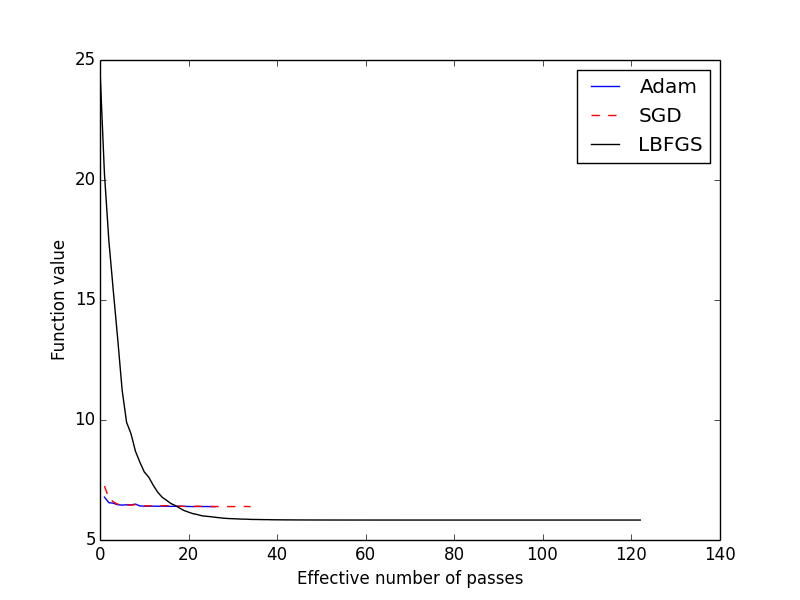
\includegraphics[width=5cm]{s1-a}}
~~
\subfigure[$\lambda =$ {\sf 1e-4}]{
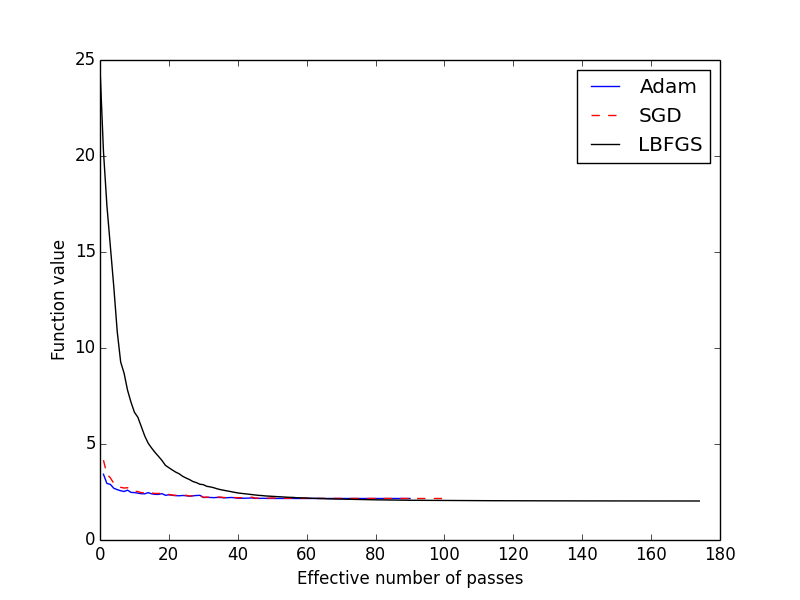
\includegraphics[width=5cm]{s1-b}}
~~
\subfigure[$\lambda =$ {\sf 1e-6}]{
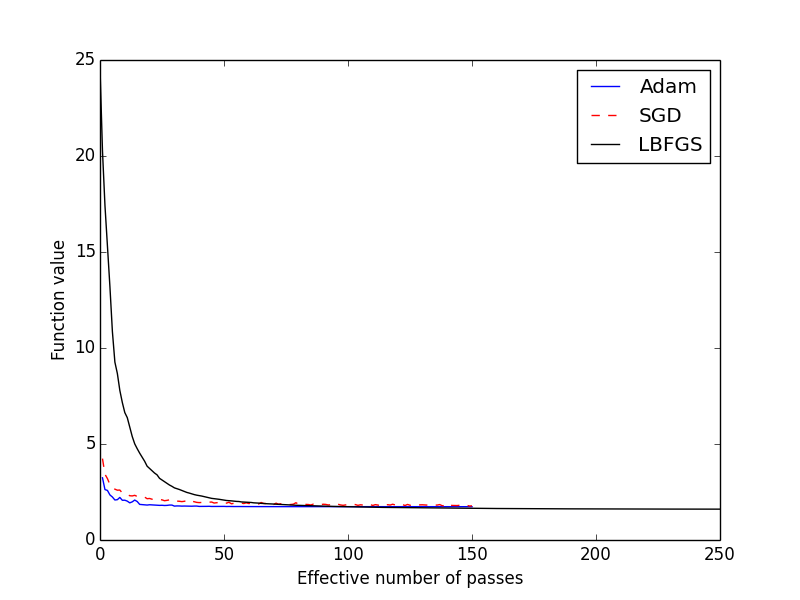
\includegraphics[width=5cm]{s1-c}}
\caption{Comparison of LBFGS, SGD, and ADAM over $\lambda \in \{${\sf 1e-2, 1e-4, 1e-6}\}.}
\label{fig:compare_sgd}
\end{figure}

\rule{\paperwidth}{0.6pt}
{\bf Answer S1.}
%

{\bf S1.1 Observations from loss plot}

We find that from the observed global minimum values of $\{6.38, 2.12, 1.61\}$ for the values of $\lambda$ = \{1e{-2}, 1e{-4}, 1e{-6}\} respectively, the stochastic optimization algorithms reach the same values, or are close to it.

Due to the use of a cyclic learning rate with Adam + AMSGrad, we observe a more erratic learning curve for that optimizer, which is due the cyclic increase of the learning rate from the triangular waveform schedule. 

In addition, we also observe cases where SGD does worse than Adam, especially in the case where $\lambda = 1e-6$. In this case, the global minima is \textit{1.61}, however Adam only approaches \textit{1.73} and SGD only approaches \textit{1.77}. We can observe during the final stages of 150 epochs of training, that the average gradient value is in the magnitude of \textit{1e-8}, and therefore this observation is due to simply insufficient training.

{\bf Question S2.}
What is your general experience of tuning the parameters of the solvers in {\bf Question S1}?
You do not need to be exhaustive, and just briefly describe what you tried and what you found.

\rule{\paperwidth}{0.6pt}
{\bf Answer S2.}
%

{\bf S2.1 Stochastic Gradient Descent with Nesterov Momentum}

We utilize Nesterov Momentum with Stochastic Gradient Descent to increase the speed of convergence on all of our models, with the default \textit{momentum} hyperparameter value of $\gamma$ to be \textit{0.9}. 

For the learning rate decay schedule, we chose a custom exponential decay schedule, with a \textit{rate} value of $0.99$ multiplied by the previous learning rate at the end of each iteration. As the optimization procedure must be performed for large number of iterations for smaller values of $\lambda$, we cap the minimum learning rate to be a dynamic variable \textit{min\_lr}, whose initial value is determined by observing the loss curve for the first 10 epochs. We compute the objective function's value every epoch, and maintain a history of the past three values. If we find that the loss has not decreased in the past three epochs, we halve \textit{min\_lr}. This causes a dynamic reduction of the current learning rate which attempts to use finer learning rate if stagnation occurs. 

We opt to break out of the optimization loop if the loss value is lesser than a certain \textit{threshold}, which is determined by observing the loss value over a predetermined number of epochs over the entire dataset.

We observe that SGD + Momentum is very sensitive to the choice of the initial learning rate and the schedule which updates it. More so than any other choice of $\gamma$ for momentum, or whether we chose to use Nesterov Momentum or not, the key hyperparameter was learning rate. Next to this, choosing an appropriate learning rate schedule was highly important as well. Choosing an exponential decay factor too high caused divergence, and very low factors caused very slow learning.

{\bf S2.2 Adam \& AMSGrad}

We utilize the Adam optimizer with the \textit{AMSGrad} correction from the paper \href{https://openreview.net/forum?id=ryQu7f-RZ}{\textit{On the Convergence of Adam and Beyond}}. We opt to use the default hyperparameters of Adam, mainly $\beta_1 = 0.9, \beta_2 = 0.999, \epsilon = 1e{-8}$, having searched for different combinations of $\beta_2$ to improve convergence speed.

For the learning rate decay schedule, we use a cyclic learning rate schedule, with a linear triangular waveform determining the increase and decrease of the base learning rate. For the cyclic learning rate function, we determine an appropriate value of \textit{stepsize, minimum learning rate and maximum learning rate} that is chosen via careful observation of the loss plot in the first 20 epochs. We still follow the learning rate decay pattern as SGD + Momentum, and also cap the learning rates to a dynamic minimum and maximum value for the cyclic learning rate, using the same methodology as used in SGD.

We opt to break out of the optimization loop if the loss value is lesser than a certain \textit{threshold}, which is determined by observing the loss value over a predetermined number of epochs over the entire dataset.

We observed that choosing an appropriate learning rate for Adam was much less of an issue as compared to SGD, and the cyclic learning rate schedule allowed for faster optimization overall compared to SGD in some cases. We attempted to use different values of $\beta_2 = {0.99, 0.999}$ and found that even though we use AMSGrad stabilization, there was no marked improvement in the overall convergence speed or value over Adam in the beginning of training. It is only near the end, that AMSGrad's stability is beneficial, whereas Adam rapidly fluctuates as it reaches close to the global minima.

{\bf Question S3.}
Fix the value of $\lambda$ to what you used in {\bf Question P3},
whose results were given in Figures \ref{fig:letter_err} and \ref{fig:word_err}.
Re-produce Figure \ref{fig:word_err} (word-wise error) but do \emph{not} include the training error any more.
Instead, include the word-wise test error of LBFGS, SGD, and ADAM.
Now it should look like Figure \ref{fig:compare_word_err}.

\begin{figure}[t]
\centering
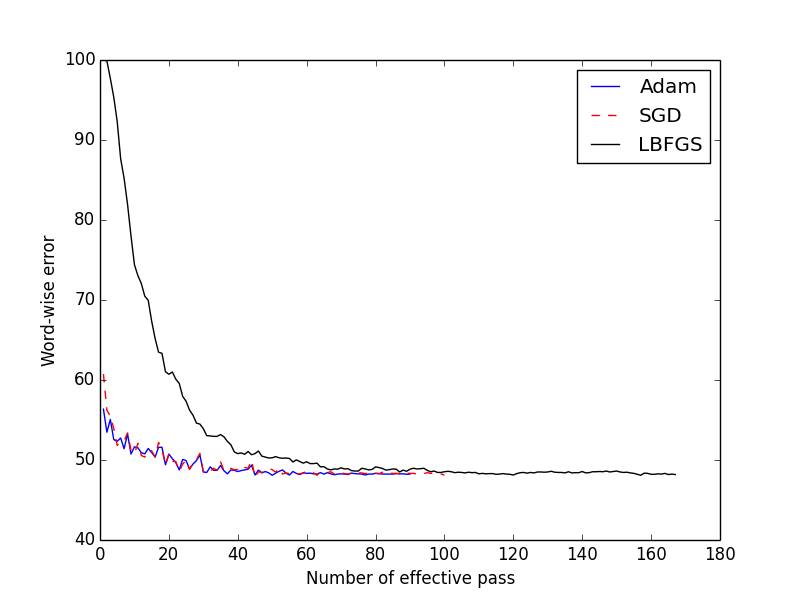
\includegraphics[width=5cm]{s3}
\caption{Comparison of word-wise error on the test data for $\lambda=$1e-4.}
\label{fig:compare_word_err}
\end{figure}

What conclusions can be drawn from the plot?


\rule{\paperwidth}{0.6pt}
{\bf Answer S3}

The primary observation is the sample_dataset wise efficiency of both stochastic optimization algorithms during training. Both SGD and ADAM quickly minimize the objective function using gradients from individual training examples, such that within one epoch, they are able to obtain a much lower word error as compared to LBFGS which performs a single update using average of the gradients over an entire training set.

We can also see that ADAM and SGD both converge near the same global optima in approximately 60 epochs, whereas the actual global minima is reached by LBFGS after approximately 150 epochs of training. Roughly, this corresponds to a sample_dataset efficiency ratio of 2.5 for the stochastic optimizers over the LBFGS optimizer.

{\bf Extra credit [15 pt].} 
In SGD and ADAM, although considerable computational savings have been achieved by using stochastic gradient based on a single randomly sampled word,
the gradient on that word is still computed exactly via message passing.
This is fine for linear chain because exact inference is not hard.
However, let us just assume that we can only do sampling (e.g., MCMC),
and therefore two levels of stochasticity have to be in place: 
randomly sampled word and approximate inference.

Now add three curves to Figure \ref{fig:compare_word_err} using ADAM+MCMC,
with the number of samples varied from low to medium to high.
You need to properly choose the exact number for ``low", ``medium", and ``high" to make the result more illustrative.
How should we change the definition of ``number of effective pass" to account for the number of samples?
For a randomly sampled word with $m$ characters, 
let us think of the message-passing based exact inference as drawing $m$ samples.

\section{Appendix}

When plotting the comparison between LBFGS, SGD, and ADAM over $\lambda \in \{${\sf 1e-2, 1e-4, 1e-6}\}, we lose the illustrative difference between Adam and SGD due to the scale issue introduced by including the LBFGS curve. Therefore, we have included the following graphs where we have separated Adam \& SGD into one graph and LBFGS into another for all three $\lambda$ values.

\begin{figure}[!htb]
\centering
\subfigure[$\lambda =$ {\sf 1e-2}]{
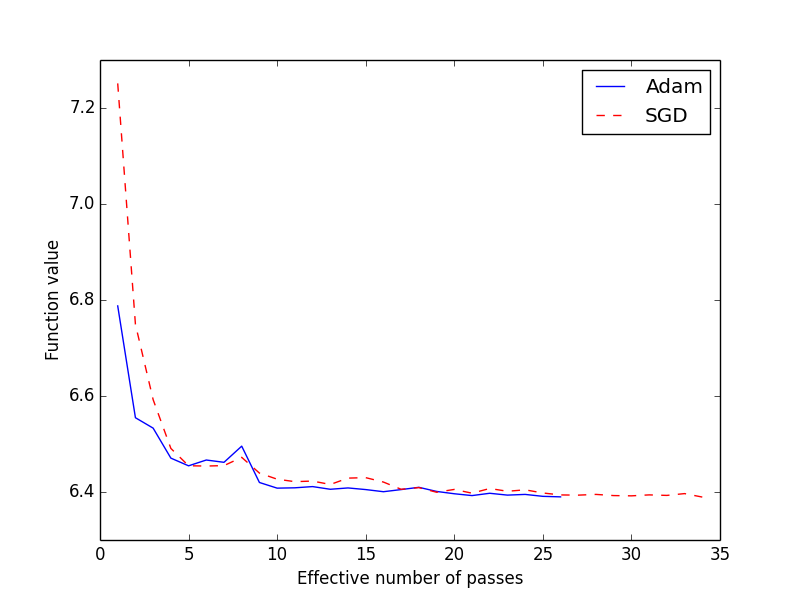
\includegraphics[width=5cm]{s1-a2}}
~~
\subfigure[$\lambda =$ {\sf 1e-4}]{
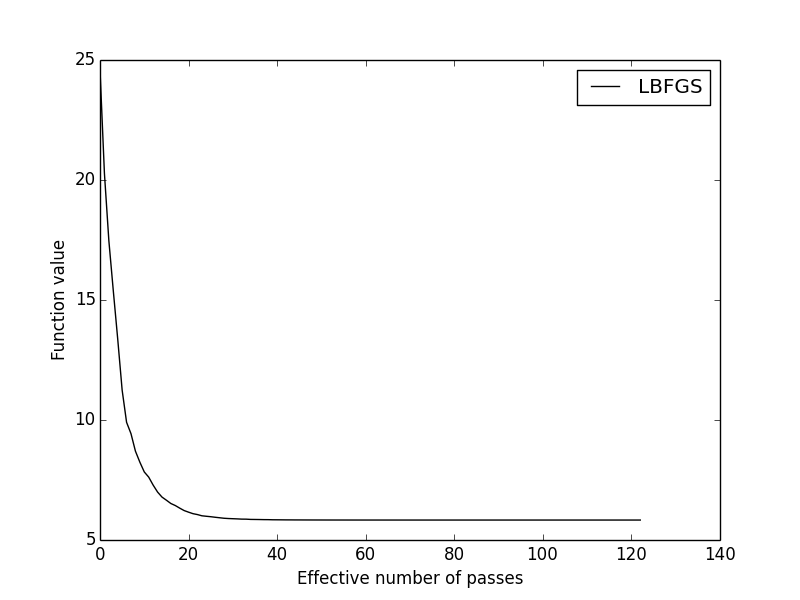
\includegraphics[width=5cm]{s1-a3}}
~~
\caption{Comparison of LBFGS vs SGD and ADAM for $\lambda \in \{${\sf 1e-2}\}.}
\label{fig:compare_sgd}
\end{figure}

\begin{figure}[!htb]
\centering
\subfigure[$\lambda =$ {\sf 1e-2}]{
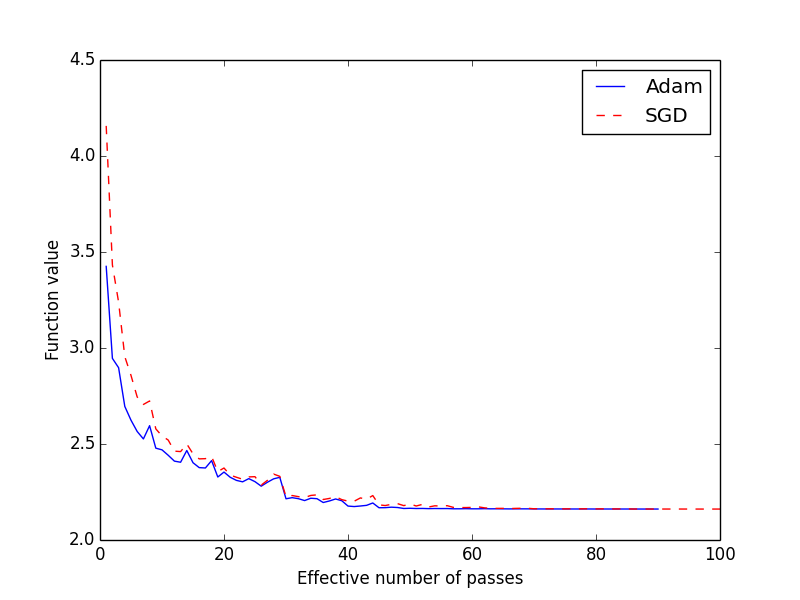
\includegraphics[width=5cm]{s1-b2}}
~~
\subfigure[$\lambda =$ {\sf 1e-4}]{
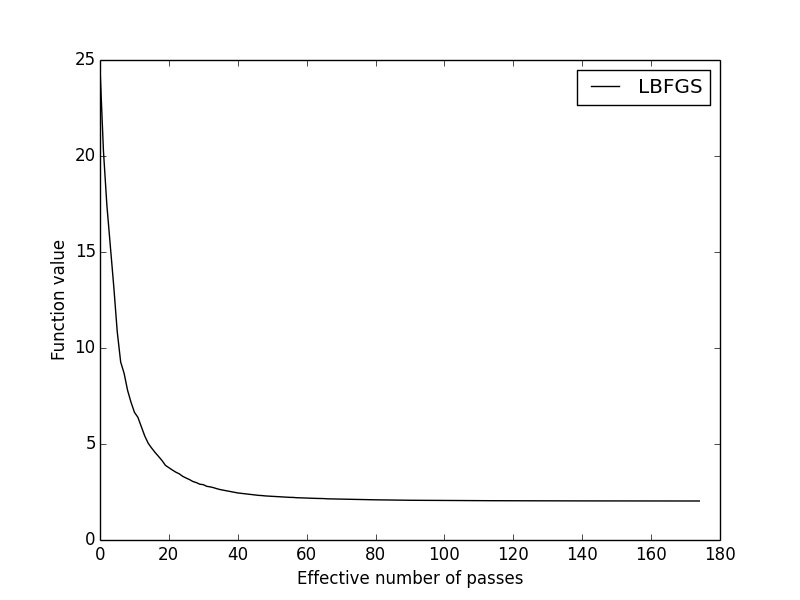
\includegraphics[width=5cm]{s1-b3}}
~~
\caption{Comparison of LBFGS vs SGD and ADAM for $\lambda \in \{${\sf 1e-4}\}.}
\label{fig:compare_sgd}
\end{figure}

\begin{figure}[!htb]
\centering
\subfigure[$\lambda =$ {\sf 1e-2}]{
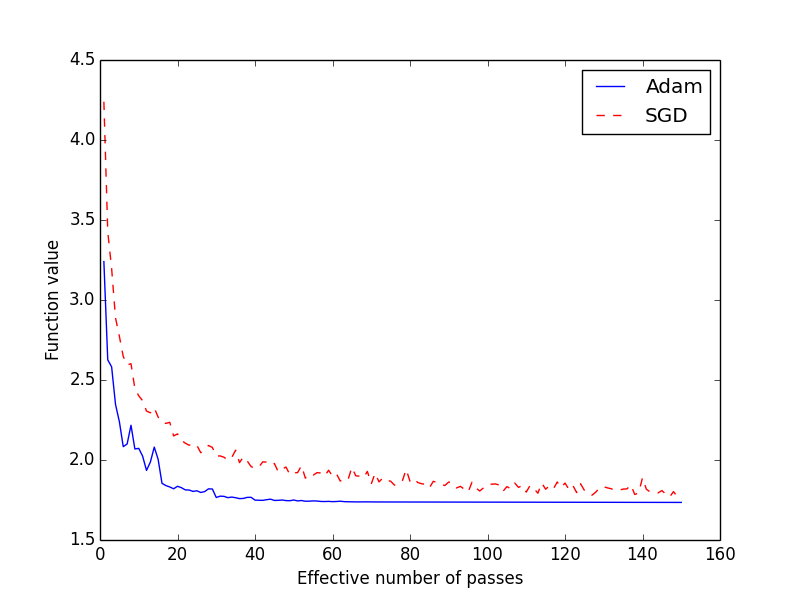
\includegraphics[width=5cm]{s1-c2}}
~~
\subfigure[$\lambda =$ {\sf 1e-4}]{
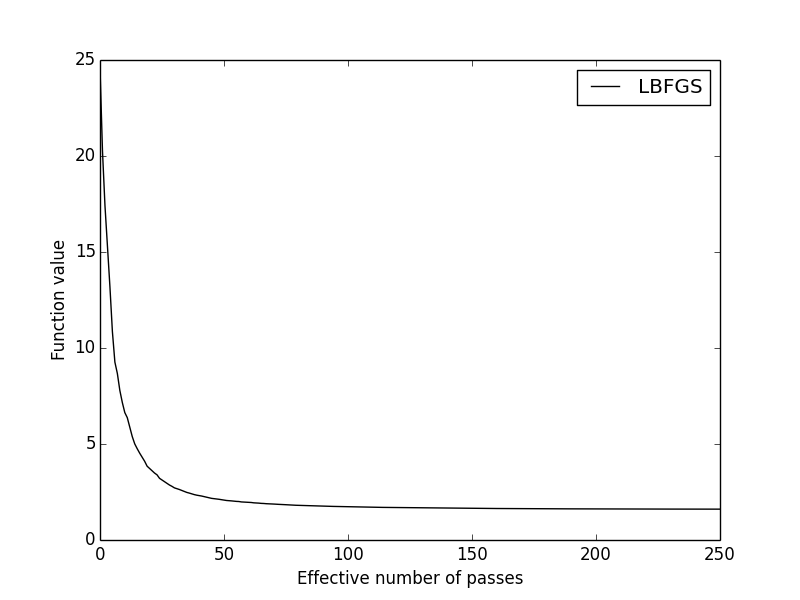
\includegraphics[width=5cm]{s1-c3}}
~~
\caption{Comparison of LBFGS vs SGD and ADAM for $\lambda \in \{${\sf 1e-6}\}.}
\label{fig:compare_sgd}
\end{figure}

\end{document}
